% !TEX root = ../sethomas_thesis_main.tex

\chapter{Sizing Methodology for Integrated SMA Actuators}\label{chap:design-methodology}
% In this chapter, a novel design methodology is present. Here, the traditional SMA actuators are adapted such that the various building blocks presented in \cref{chap:sma-actuator-design} are integrated together. The basic working principle of the new design methodology consists of taking the traditional building blocks of SMA actuator design and create novel building blocks that are combined to create more integrated solutions. This method allows the design of SMA actuators that are more integrated and further improves the, already, high work volume density of the smart material. Furthermore, the modelling techniques employed in \cref{chap:sma-model} are adapted based on the novel design methodology such that the novel systems described can be adequately sized for any application.

% Goal : Show a general way to size SMA actuators with novel biasing elements
% Problem : Biasing mechanisms can be replaced / integrated into motion conversion systems (flexural systems)
%           No way to size SMA in these systems
% Solution : Analytical model and how to modify such that you can integrate flexural systems

\section{Introduction}
% Throwback to previous chapter
% Present the push towards to miniaturisation
% State of the art of Motion conversion systems
In the past few decades, there has been a growing need for miniaturisation. Modern devices have come to require actuators that are compact and lightweight. As mentioned previously, since SMAs have been known to show the highest volumetric work density, they have been increasingly used in applications where compactness and low weight are required.

As previously presented in \cref{chap:sma-actuator-design}, SMA actuators require an active element, a biasing element and a kinematic stage for motion control. These components, usually discrete elements, when combined together create an SMA actuator that can preform a specific reversible work, such as gripping or crawling motions\todocite. With the objective of miniaturisation, most work has been conducted into rendering these individual components as compact and lightweight as possible\todocite. But the fact that these stages are discrete, lowers the overall volumetric work density of the complete actuator. Furthermore, as multiple systems are needed, the actuator also requires various pieces and assembly increasing the complexity and decreasing the compactness.

% Figure about SMA actuator with flexure mechanism

Recently, there has been a shift in creating novel motion control mechanisms using flexure-based mechanisms. These flexures are multiple compliant elements designed so as to only be compliant in specific degrees of freedom while being rigid in the others. These mechanisms, which can be fabricated using a monolithic piece of material, are lightweight and require virtually no assembly. These flexural stages, when paired with SMAs, have greatly increased the overall work density of the traditional SMA actuators\todocite.

% Figure about flexure based mechanism

These flexure-based mechanisms are still often integrated into the SMA actuators as discrete mechanisms. In this chapter, the concept of integrating the biasing element as a flexural mechanism is explored. In this case, the kinematic stage and the biasing element are combined and are no longer discrete systems within the mechanism. Some research has been shown to take into account flexure mechanisms in SMA actuators but they lack a suitable sizing strategy due to the complexity of the shape memory effect and the nonlinear nature of flexures\todocite. Thus, in this chapter, this novel design methodology is presented and analysed using an analytical model.

\section{Adapted Design Concept}
% Present new design concept and methodology
As mentioned previously, most SMA actuators are composed of an active element, a biasing element and a kinematic stage charged with converting the linear output of the actuator into a more complex one. In general, these elements are discrete components ranging from SMA coils, passive biasing springs and the kinematic stage comprised of hinges and linear slides. As presented in \cref{fig:building-blocks-pt}, the design methodology consists of integrating the kinematic stage and the biasing element.

% Figure about combined concept diagram
\begin{figure}[h] % t for top of the page, H could be put to impose the position of the float
  \centering
  \begin{tikzpicture}
    \node[anchor=south west,inner sep=0] (graph) at (0,0) {
\includegraphics[trim={0 0 0 0},clip, width=0.8\textwidth]{images/chap4/hexgon-base-layer-intersect-pt.pdf}};
	% Insert a relative reference based on image dimensions
    \begin{scope}[x={(graph.south east)},y={(graph.north west)}]
    \node[] at (0.19, 0.5) {\textcolor{white}{\large Active Element}};
    \node[] at (0.52, 0.75) {\textcolor{white}{\large Kinematic Stage}};
    \node[] at (0.5, 0.25) {\textcolor{white}{\large Control Stage}};
    \node[] at (0.82, 0.52) {\textcolor{white}{\large Biasing Element}};
    \end{scope}
    \end{tikzpicture}
  \caption{Diagram of the adapted building blocks of the SMA actuator.}
  \label{fig:building-blocks-pt}
\end{figure}

This integration can be accomplished with the use of flexure-based mechanisms. Generally, flexures have been used in creating an alternative solution for traditional hinges and linear slides. These flexures are comprised of cantilever beams which allows the mechanism to be compliant in a specific degree of freedom while being rigid in the others. The advantages of such a system is that when adequately design can result in a kinematic stage that is lightweight, lacks any assembly and has high precision.

% Figure with example of flexure mechanism

The main drawback to such a system compared to traditional bearings is the inherent stiffness of the mechanism. As these flexures are composed of compliant beams, the rigidity of the beam must be taken into account. In the case of an SMA actuator, this rigidity of the compliant structure can be harnessed as the biasing element. This implies that by pairing the active SMA element with a flexure, the kinematic stage and the biasing element can be combined. This novel approach can be used to create biased SMA actuators that are precise, lightweight and with a limited number of pieces to be assembled.

\section{Challenges of the Approach}
% Present the challenges regarding the sizing of such a methodology
Due to the complex nature of the shape memory effect, the principle challenge when it comes to designing such SMA actuators is the difficulty in sizing the active SMA based on the flexure mechanism. Based on the configuration of the flexural stage, this mechanism can present highly nonlinear behaviour as well. When paired with an SMA wire or coil, this can results in unintended behaviours or secondary operating points.

% Show example of literature with lack of sizing of SMA
Recently there has been research such as the work by \cite{maffiodo_three-fingered_2017} that shows the advantages of pairing SMA wires with flexure-based structures. As with this case, the sizing of the SMA element is disregarding and the biasing advantage of the flexure is neglected.
% Importance of sizing SMA (thermals)

In the case of grippers and mesoscale actuators where the SMA element is passively cooled, the accurate sizing of the SMA is important. In designs, where passive cooling is used, the geometry of the active element is critical as the shape and structure of the active element is directly related to the cooling times. In the case of SMA coils and wires, thinner diameters imply a shorter cooling time. These thinner wires, however, result in smaller forces when heated. This implies that by accurately sizing the SMA element for the biasing flexure, the actuator can be made as thin as possible while still being able to deform the flexure during heating. Thus, by adapting the traditional sizing methodology of bias-spring SMA actuators for flexure-based designs, the SMA actuator can be designed with faster response times.

\section{Adapting the Simplified Models}
% Combining biasing element and motion conversion system
In \cref{sec:simplified-sma-model}, a simplified model of the SMAs are used to size the active element for bias-spring and antagonistic SMA actuators. In the traditional sizing strategy, a simplified linear model of the SMA and the curve of the spring are used to find the operating points of the actuator which is represented by the intersection of the two curves. This simplification allows a relatively simpler sizing of the components by abstracting the complex nonlinear behaviours of the shape memory effect.

\subsection{Passive Biasing Compliant Mechanisms}
% Adding complex systems to antagonistic SMA pairs
The compliant mechanism, as mentioned previously, acts as the biasing element and as the kinematic stage that produces the desired actuator motion. Here, the basic principle is that the inherent stiffness of the compliant flexure mechanism is harnessed to pre-load the SMA for activation. In this case, at lower temperatures, the SMA is deformed using the energy stored in the compliant mechanism while at higher temperatures, the strain recovered by the shape memory effect is used to deform the compliant mechanism. Based on the design of the compliant mechanism, the SMA actuator can be made to actuate reversibly in a single degree of freedom while being rigid in the others.

In order to size the actuator and its corresponding passive biasing compliant element, an analytical model can be devised and exploited to predict the various operating points of the final SMA actuator. A pseudo-rigid body model (PSBM) based on the work by \cite{heneinConceptionStructuresArticulees2005} can be used to devise the analytical models of the flexures. The flexure hinges are considered to behave like torsional springs with constant angular stiffness, $K_\theta$. The analytical model can be derived by considering the reaction force exerted by the mechanism on the SMA wire or coil when acting as the biasing element.

While a Newtonian approach is possible, the simplest way to compute the force is to consider the elastic potential energy stored in the flexure hinges as the mechanism deforms. This potential energy stored in one torsional spring as a function of the input displacement of the mechanism, $x$, as given by :
\begin{equation}\label{eq:flexure-pot-energy}
        U(x) = \frac{1}{2}K_{\theta} \left(\theta(x)-\theta_0 \right)^2
\end{equation}
where, in the case of a notch flexure hinge, as shown in \cref{fig:notch-flexure}, when rotating by an angle of $\theta$, has a stiffness, as described in \cite{heneinConceptionStructuresArticulees2005}, equal to:
\begin{equation}\label{eq:flexure-hinge-stiffness}
        K_{\theta} = \frac{2Ebe^{2.5}}{9\pi \sqrt{r}}
\end{equation}
Here, $E$ is the Young modulus of the material, and $e$,$b$ and $r$ the design parameters of the flexure hinge shown in \cref{fig:notch-flexure}.

\begin{figure}[h] % t for top of the page, H could be put to impose the position of the float
  \centering
  \begin{tikzpicture}
    \node[anchor=south west,inner sep=0] (graph) at (0,0) {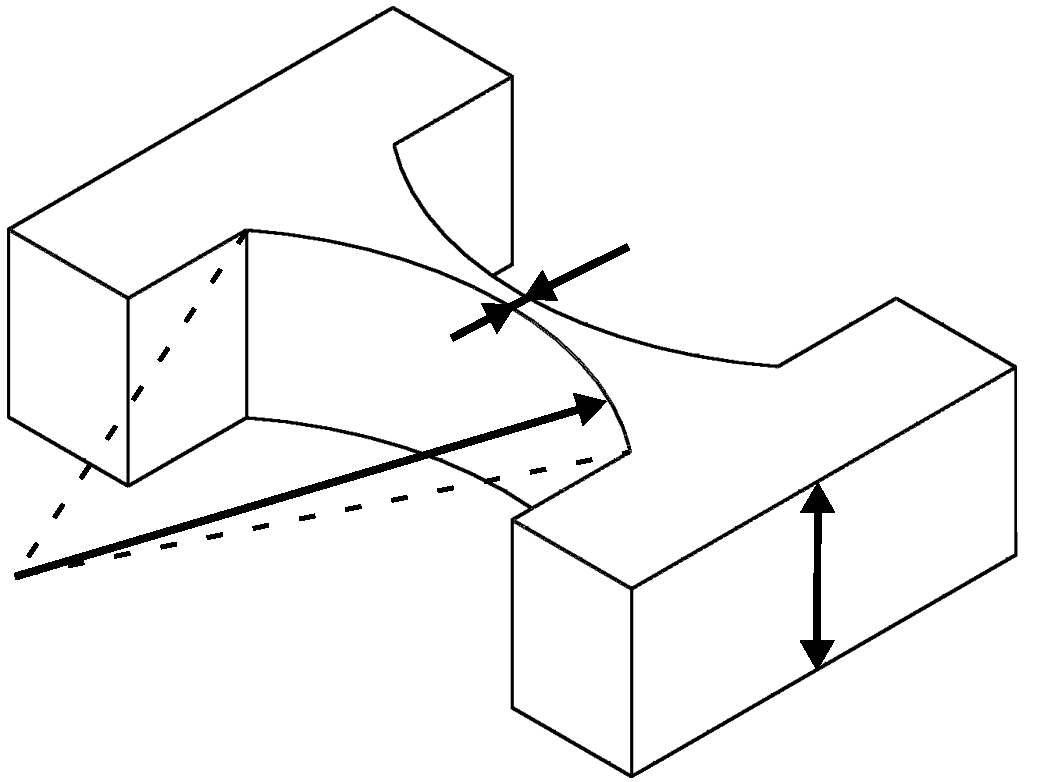
\includegraphics[width=0.4\textwidth]{images/chap4/pivot_notch.pdf}};
	% Insert a relative reference based on image dimensions
    \begin{scope}[x={(graph.south east)},y={(graph.north west)}]
        \node[] at (0.29, 0.45) {\Large $r$};
        \node[] at (0.83, 0.29) {\Large $b$};
        \node[] at (0.58, 0.73) {\Large $e$};
    \end{scope}
    \end{tikzpicture}
%   \begin{tikzpicture} % Comment to remove border
    % \node (table) [inner sep=1pt] { % Comment to remove border
  % \begin{tabular}{r@{ }l r@{ }l}
  %   {\color{myblue} \rule[2pt]{10pt}{0.5mm} } & SMA at Low Temperature & {\color{myred} \rule[2pt]{10pt}{0.5mm} } & SMA at High Temperature\\
  %   {\color{mygreen} \rule[2pt]{10pt}{0.5mm} } & Compliant Mechanism &  & \\
  % \end{tabular}
%   };% Comment to remove border
% \draw [rounded corners=.2em] (table.north west) rectangle (table.south east);% Comment to remove border
% \end{tikzpicture}% Comment to remove border
  \caption{A diagram of the notch flexure hinge.}
  \label{fig:notch-flexure}
\end{figure}

In this approach, the important relationship to obtain is the influence of the contraction of the SMA on the rotation of the hinge, $\theta(x)$. When the flexure-based system is comprised of multiple flexural hinges, the total potential energy can be calculated by the sum of the potential elastic energy of each flexure, $U_\mathrm{tot}=\sum U(x)$. The required force to deform the structure can be deduced using :
\begin{equation}\label{eq:flexure-hinge-force}
    F(\theta(x)) = \lVert -\nabla{U_\text{tot}(x)}\rVert = \frac{\partial U_\text{tot}(x)}{\partial x}
\end{equation}

%%%%%%%% WORKING PRINCIPLE FIGURE %%%%%%%%%%%
\begin{figure}[ht] % t for top of the page, H could be put to impose the position of the float
  \centering
  \begin{tikzpicture}
    \node[anchor=south west,inner sep=0] (graph) at (0,0) {\resizebox{0.7\columnwidth}{!}{%% Creator: Matplotlib, PGF backend
%%
%% To include the figure in your LaTeX document, write
%%   \input{<filename>.pgf}
%%
%% Make sure the required packages are loaded in your preamble
%%   \usepackage{pgf}
%%
%% and, on pdftex
%%   \usepackage[utf8]{inputenc}\DeclareUnicodeCharacter{2212}{-}
%%
%% or, on luatex and xetex
%%   \usepackage{unicode-math}
%%
%% Figures using additional raster images can only be included by \input if
%% they are in the same directory as the main LaTeX file. For loading figures
%% from other directories you can use the `import` package
%%   \usepackage{import}
%%
%% and then include the figures with
%%   \import{<path to file>}{<filename>.pgf}
%%
%% Matplotlib used the following preamble
%%
\begingroup%
\makeatletter%
\begin{pgfpicture}%
\pgfpathrectangle{\pgfpointorigin}{\pgfqpoint{5.994474in}{4.501709in}}%
\pgfusepath{use as bounding box, clip}%
\begin{pgfscope}%
\pgfsetbuttcap%
\pgfsetmiterjoin%
\pgfsetlinewidth{0.000000pt}%
\definecolor{currentstroke}{rgb}{0.000000,0.000000,0.000000}%
\pgfsetstrokecolor{currentstroke}%
\pgfsetstrokeopacity{0.000000}%
\pgfsetdash{}{0pt}%
\pgfpathmoveto{\pgfqpoint{0.000000in}{0.000000in}}%
\pgfpathlineto{\pgfqpoint{5.994474in}{0.000000in}}%
\pgfpathlineto{\pgfqpoint{5.994474in}{4.501709in}}%
\pgfpathlineto{\pgfqpoint{0.000000in}{4.501709in}}%
\pgfpathclose%
\pgfusepath{}%
\end{pgfscope}%
\begin{pgfscope}%
\pgfsetbuttcap%
\pgfsetmiterjoin%
\pgfsetlinewidth{0.000000pt}%
\definecolor{currentstroke}{rgb}{0.000000,0.000000,0.000000}%
\pgfsetstrokecolor{currentstroke}%
\pgfsetstrokeopacity{0.000000}%
\pgfsetdash{}{0pt}%
\pgfpathmoveto{\pgfqpoint{0.934474in}{0.705709in}}%
\pgfpathlineto{\pgfqpoint{5.894474in}{0.705709in}}%
\pgfpathlineto{\pgfqpoint{5.894474in}{4.401709in}}%
\pgfpathlineto{\pgfqpoint{0.934474in}{4.401709in}}%
\pgfpathclose%
\pgfusepath{}%
\end{pgfscope}%
\begin{pgfscope}%
\pgfpathrectangle{\pgfqpoint{0.934474in}{0.705709in}}{\pgfqpoint{4.960000in}{3.696000in}}%
\pgfusepath{clip}%
\pgfsetrectcap%
\pgfsetroundjoin%
\pgfsetlinewidth{2.007500pt}%
\definecolor{currentstroke}{rgb}{0.000000,0.447059,0.741176}%
\pgfsetstrokecolor{currentstroke}%
\pgfsetdash{}{0pt}%
\pgfpathmoveto{\pgfqpoint{0.934474in}{0.705709in}}%
\pgfpathlineto{\pgfqpoint{5.897807in}{2.554951in}}%
\pgfpathlineto{\pgfqpoint{5.897807in}{2.554951in}}%
\pgfusepath{stroke}%
\end{pgfscope}%
\begin{pgfscope}%
\pgfpathrectangle{\pgfqpoint{0.934474in}{0.705709in}}{\pgfqpoint{4.960000in}{3.696000in}}%
\pgfusepath{clip}%
\pgfsetrectcap%
\pgfsetroundjoin%
\pgfsetlinewidth{2.007500pt}%
\definecolor{currentstroke}{rgb}{0.768627,0.000000,0.047059}%
\pgfsetstrokecolor{currentstroke}%
\pgfsetdash{}{0pt}%
\pgfpathmoveto{\pgfqpoint{0.934474in}{0.705709in}}%
\pgfpathlineto{\pgfqpoint{2.589298in}{4.405043in}}%
\pgfpathlineto{\pgfqpoint{2.589298in}{4.405043in}}%
\pgfusepath{stroke}%
\end{pgfscope}%
\begin{pgfscope}%
\pgfpathrectangle{\pgfqpoint{0.934474in}{0.705709in}}{\pgfqpoint{4.960000in}{3.696000in}}%
\pgfusepath{clip}%
\pgfsetrectcap%
\pgfsetroundjoin%
\pgfsetlinewidth{2.007500pt}%
\definecolor{currentstroke}{rgb}{0.145098,0.560784,0.105882}%
\pgfsetstrokecolor{currentstroke}%
\pgfsetdash{}{0pt}%
\pgfpathmoveto{\pgfqpoint{0.934474in}{3.165443in}}%
\pgfpathlineto{\pgfqpoint{1.097441in}{3.122127in}}%
\pgfpathlineto{\pgfqpoint{1.255152in}{3.079456in}}%
\pgfpathlineto{\pgfqpoint{1.407606in}{3.037465in}}%
\pgfpathlineto{\pgfqpoint{1.560059in}{2.994704in}}%
\pgfpathlineto{\pgfqpoint{1.707256in}{2.952645in}}%
\pgfpathlineto{\pgfqpoint{1.849196in}{2.911329in}}%
\pgfpathlineto{\pgfqpoint{1.985878in}{2.870798in}}%
\pgfpathlineto{\pgfqpoint{2.122561in}{2.829494in}}%
\pgfpathlineto{\pgfqpoint{2.253986in}{2.789007in}}%
\pgfpathlineto{\pgfqpoint{2.380155in}{2.749384in}}%
\pgfpathlineto{\pgfqpoint{2.506323in}{2.708978in}}%
\pgfpathlineto{\pgfqpoint{2.627235in}{2.669475in}}%
\pgfpathlineto{\pgfqpoint{2.742889in}{2.630932in}}%
\pgfpathlineto{\pgfqpoint{2.858544in}{2.591601in}}%
\pgfpathlineto{\pgfqpoint{2.968941in}{2.553277in}}%
\pgfpathlineto{\pgfqpoint{3.074082in}{2.516024in}}%
\pgfpathlineto{\pgfqpoint{3.179222in}{2.477988in}}%
\pgfpathlineto{\pgfqpoint{3.279105in}{2.441082in}}%
\pgfpathlineto{\pgfqpoint{3.378989in}{2.403373in}}%
\pgfpathlineto{\pgfqpoint{3.473615in}{2.366860in}}%
\pgfpathlineto{\pgfqpoint{3.568242in}{2.329526in}}%
\pgfpathlineto{\pgfqpoint{3.657611in}{2.293460in}}%
\pgfpathlineto{\pgfqpoint{3.741723in}{2.258751in}}%
\pgfpathlineto{\pgfqpoint{3.825836in}{2.223248in}}%
\pgfpathlineto{\pgfqpoint{3.904691in}{2.189193in}}%
\pgfpathlineto{\pgfqpoint{3.983546in}{2.154337in}}%
\pgfpathlineto{\pgfqpoint{4.057145in}{2.121031in}}%
\pgfpathlineto{\pgfqpoint{4.130743in}{2.086922in}}%
\pgfpathlineto{\pgfqpoint{4.199084in}{2.054477in}}%
\pgfpathlineto{\pgfqpoint{4.267426in}{2.021232in}}%
\pgfpathlineto{\pgfqpoint{4.335767in}{1.987125in}}%
\pgfpathlineto{\pgfqpoint{4.398851in}{1.954815in}}%
\pgfpathlineto{\pgfqpoint{4.461935in}{1.921647in}}%
\pgfpathlineto{\pgfqpoint{4.519763in}{1.890428in}}%
\pgfpathlineto{\pgfqpoint{4.577590in}{1.858363in}}%
\pgfpathlineto{\pgfqpoint{4.630160in}{1.828419in}}%
\pgfpathlineto{\pgfqpoint{4.682730in}{1.797654in}}%
\pgfpathlineto{\pgfqpoint{4.735300in}{1.765996in}}%
\pgfpathlineto{\pgfqpoint{4.782614in}{1.736674in}}%
\pgfpathlineto{\pgfqpoint{4.829927in}{1.706493in}}%
\pgfpathlineto{\pgfqpoint{4.877240in}{1.675373in}}%
\pgfpathlineto{\pgfqpoint{4.919296in}{1.646847in}}%
\pgfpathlineto{\pgfqpoint{4.961352in}{1.617429in}}%
\pgfpathlineto{\pgfqpoint{5.003409in}{1.587030in}}%
\pgfpathlineto{\pgfqpoint{5.040208in}{1.559543in}}%
\pgfpathlineto{\pgfqpoint{5.077007in}{1.531142in}}%
\pgfpathlineto{\pgfqpoint{5.113806in}{1.501728in}}%
\pgfpathlineto{\pgfqpoint{5.145348in}{1.475621in}}%
\pgfpathlineto{\pgfqpoint{5.176890in}{1.448599in}}%
\pgfpathlineto{\pgfqpoint{5.208432in}{1.420555in}}%
\pgfpathlineto{\pgfqpoint{5.239975in}{1.391365in}}%
\pgfpathlineto{\pgfqpoint{5.266260in}{1.366055in}}%
\pgfpathlineto{\pgfqpoint{5.292545in}{1.339736in}}%
\pgfpathlineto{\pgfqpoint{5.318830in}{1.312276in}}%
\pgfpathlineto{\pgfqpoint{5.339858in}{1.289378in}}%
\pgfpathlineto{\pgfqpoint{5.360886in}{1.265545in}}%
\pgfpathlineto{\pgfqpoint{5.381914in}{1.240651in}}%
\pgfpathlineto{\pgfqpoint{5.402942in}{1.214540in}}%
\pgfpathlineto{\pgfqpoint{5.423970in}{1.187015in}}%
\pgfpathlineto{\pgfqpoint{5.439741in}{1.165291in}}%
\pgfpathlineto{\pgfqpoint{5.455512in}{1.142487in}}%
\pgfpathlineto{\pgfqpoint{5.471284in}{1.118426in}}%
\pgfpathlineto{\pgfqpoint{5.487055in}{1.092871in}}%
\pgfpathlineto{\pgfqpoint{5.502826in}{1.065507in}}%
\pgfpathlineto{\pgfqpoint{5.513340in}{1.046044in}}%
\pgfpathlineto{\pgfqpoint{5.523854in}{1.025398in}}%
\pgfpathlineto{\pgfqpoint{5.534368in}{1.003323in}}%
\pgfpathlineto{\pgfqpoint{5.544882in}{0.979474in}}%
\pgfpathlineto{\pgfqpoint{5.555396in}{0.953339in}}%
\pgfpathlineto{\pgfqpoint{5.565910in}{0.924098in}}%
\pgfpathlineto{\pgfqpoint{5.571167in}{0.907898in}}%
\pgfpathlineto{\pgfqpoint{5.576424in}{0.890282in}}%
\pgfpathlineto{\pgfqpoint{5.581681in}{0.870796in}}%
\pgfpathlineto{\pgfqpoint{5.586938in}{0.848678in}}%
\pgfpathlineto{\pgfqpoint{5.592195in}{0.822443in}}%
\pgfpathlineto{\pgfqpoint{5.597452in}{0.788253in}}%
\pgfpathlineto{\pgfqpoint{5.602709in}{0.705709in}}%
\pgfpathlineto{\pgfqpoint{5.602709in}{0.705709in}}%
\pgfusepath{stroke}%
\end{pgfscope}%
\begin{pgfscope}%
\pgfpathrectangle{\pgfqpoint{0.934474in}{0.705709in}}{\pgfqpoint{4.960000in}{3.696000in}}%
\pgfusepath{clip}%
\pgfsetbuttcap%
\pgfsetroundjoin%
\pgfsetlinewidth{0.803000pt}%
\definecolor{currentstroke}{rgb}{0.690196,0.690196,0.690196}%
\pgfsetstrokecolor{currentstroke}%
\pgfsetdash{{0.800000pt}{1.320000pt}}{0.000000pt}%
\pgfpathmoveto{\pgfqpoint{0.934474in}{0.705709in}}%
\pgfpathlineto{\pgfqpoint{0.934474in}{4.401709in}}%
\pgfusepath{stroke}%
\end{pgfscope}%
\begin{pgfscope}%
\pgfsetbuttcap%
\pgfsetroundjoin%
\definecolor{currentfill}{rgb}{0.000000,0.000000,0.000000}%
\pgfsetfillcolor{currentfill}%
\pgfsetlinewidth{0.803000pt}%
\definecolor{currentstroke}{rgb}{0.000000,0.000000,0.000000}%
\pgfsetstrokecolor{currentstroke}%
\pgfsetdash{}{0pt}%
\pgfsys@defobject{currentmarker}{\pgfqpoint{0.000000in}{-0.048611in}}{\pgfqpoint{0.000000in}{0.000000in}}{%
\pgfpathmoveto{\pgfqpoint{0.000000in}{0.000000in}}%
\pgfpathlineto{\pgfqpoint{0.000000in}{-0.048611in}}%
\pgfusepath{stroke,fill}%
}%
\begin{pgfscope}%
\pgfsys@transformshift{0.934474in}{0.705709in}%
\pgfsys@useobject{currentmarker}{}%
\end{pgfscope}%
\end{pgfscope}%
\begin{pgfscope}%
\definecolor{textcolor}{rgb}{0.000000,0.000000,0.000000}%
\pgfsetstrokecolor{textcolor}%
\pgfsetfillcolor{textcolor}%
\pgftext[x=0.934474in,y=0.608487in,,top]{\color{textcolor}\rmfamily\fontsize{16.000000}{19.200000}\selectfont 0}%
\end{pgfscope}%
\begin{pgfscope}%
\pgfpathrectangle{\pgfqpoint{0.934474in}{0.705709in}}{\pgfqpoint{4.960000in}{3.696000in}}%
\pgfusepath{clip}%
\pgfsetbuttcap%
\pgfsetroundjoin%
\pgfsetlinewidth{0.803000pt}%
\definecolor{currentstroke}{rgb}{0.690196,0.690196,0.690196}%
\pgfsetstrokecolor{currentstroke}%
\pgfsetdash{{0.800000pt}{1.320000pt}}{0.000000pt}%
\pgfpathmoveto{\pgfqpoint{4.351622in}{0.705709in}}%
\pgfpathlineto{\pgfqpoint{4.351622in}{4.401709in}}%
\pgfusepath{stroke}%
\end{pgfscope}%
\begin{pgfscope}%
\pgfsetbuttcap%
\pgfsetroundjoin%
\definecolor{currentfill}{rgb}{0.000000,0.000000,0.000000}%
\pgfsetfillcolor{currentfill}%
\pgfsetlinewidth{0.803000pt}%
\definecolor{currentstroke}{rgb}{0.000000,0.000000,0.000000}%
\pgfsetstrokecolor{currentstroke}%
\pgfsetdash{}{0pt}%
\pgfsys@defobject{currentmarker}{\pgfqpoint{0.000000in}{-0.048611in}}{\pgfqpoint{0.000000in}{0.000000in}}{%
\pgfpathmoveto{\pgfqpoint{0.000000in}{0.000000in}}%
\pgfpathlineto{\pgfqpoint{0.000000in}{-0.048611in}}%
\pgfusepath{stroke,fill}%
}%
\begin{pgfscope}%
\pgfsys@transformshift{4.351622in}{0.705709in}%
\pgfsys@useobject{currentmarker}{}%
\end{pgfscope}%
\end{pgfscope}%
\begin{pgfscope}%
\definecolor{textcolor}{rgb}{0.000000,0.000000,0.000000}%
\pgfsetstrokecolor{textcolor}%
\pgfsetfillcolor{textcolor}%
\pgftext[x=4.351622in,y=0.608487in,,top]{\color{textcolor}\rmfamily\fontsize{16.000000}{19.200000}\selectfont \(\displaystyle x_1\)}%
\end{pgfscope}%
\begin{pgfscope}%
\pgfpathrectangle{\pgfqpoint{0.934474in}{0.705709in}}{\pgfqpoint{4.960000in}{3.696000in}}%
\pgfusepath{clip}%
\pgfsetbuttcap%
\pgfsetroundjoin%
\pgfsetlinewidth{0.803000pt}%
\definecolor{currentstroke}{rgb}{0.690196,0.690196,0.690196}%
\pgfsetstrokecolor{currentstroke}%
\pgfsetdash{{0.800000pt}{1.320000pt}}{0.000000pt}%
\pgfpathmoveto{\pgfqpoint{1.912469in}{0.705709in}}%
\pgfpathlineto{\pgfqpoint{1.912469in}{4.401709in}}%
\pgfusepath{stroke}%
\end{pgfscope}%
\begin{pgfscope}%
\pgfsetbuttcap%
\pgfsetroundjoin%
\definecolor{currentfill}{rgb}{0.000000,0.000000,0.000000}%
\pgfsetfillcolor{currentfill}%
\pgfsetlinewidth{0.803000pt}%
\definecolor{currentstroke}{rgb}{0.000000,0.000000,0.000000}%
\pgfsetstrokecolor{currentstroke}%
\pgfsetdash{}{0pt}%
\pgfsys@defobject{currentmarker}{\pgfqpoint{0.000000in}{-0.048611in}}{\pgfqpoint{0.000000in}{0.000000in}}{%
\pgfpathmoveto{\pgfqpoint{0.000000in}{0.000000in}}%
\pgfpathlineto{\pgfqpoint{0.000000in}{-0.048611in}}%
\pgfusepath{stroke,fill}%
}%
\begin{pgfscope}%
\pgfsys@transformshift{1.912469in}{0.705709in}%
\pgfsys@useobject{currentmarker}{}%
\end{pgfscope}%
\end{pgfscope}%
\begin{pgfscope}%
\definecolor{textcolor}{rgb}{0.000000,0.000000,0.000000}%
\pgfsetstrokecolor{textcolor}%
\pgfsetfillcolor{textcolor}%
\pgftext[x=1.912469in,y=0.608487in,,top]{\color{textcolor}\rmfamily\fontsize{16.000000}{19.200000}\selectfont \(\displaystyle x_2\)}%
\end{pgfscope}%
\begin{pgfscope}%
\pgfpathrectangle{\pgfqpoint{0.934474in}{0.705709in}}{\pgfqpoint{4.960000in}{3.696000in}}%
\pgfusepath{clip}%
\pgfsetbuttcap%
\pgfsetroundjoin%
\pgfsetlinewidth{0.803000pt}%
\definecolor{currentstroke}{rgb}{0.690196,0.690196,0.690196}%
\pgfsetstrokecolor{currentstroke}%
\pgfsetdash{{0.800000pt}{1.320000pt}}{0.000000pt}%
\pgfpathmoveto{\pgfqpoint{5.602709in}{0.705709in}}%
\pgfpathlineto{\pgfqpoint{5.602709in}{4.401709in}}%
\pgfusepath{stroke}%
\end{pgfscope}%
\begin{pgfscope}%
\pgfsetbuttcap%
\pgfsetroundjoin%
\definecolor{currentfill}{rgb}{0.000000,0.000000,0.000000}%
\pgfsetfillcolor{currentfill}%
\pgfsetlinewidth{0.803000pt}%
\definecolor{currentstroke}{rgb}{0.000000,0.000000,0.000000}%
\pgfsetstrokecolor{currentstroke}%
\pgfsetdash{}{0pt}%
\pgfsys@defobject{currentmarker}{\pgfqpoint{0.000000in}{-0.048611in}}{\pgfqpoint{0.000000in}{0.000000in}}{%
\pgfpathmoveto{\pgfqpoint{0.000000in}{0.000000in}}%
\pgfpathlineto{\pgfqpoint{0.000000in}{-0.048611in}}%
\pgfusepath{stroke,fill}%
}%
\begin{pgfscope}%
\pgfsys@transformshift{5.602709in}{0.705709in}%
\pgfsys@useobject{currentmarker}{}%
\end{pgfscope}%
\end{pgfscope}%
\begin{pgfscope}%
\definecolor{textcolor}{rgb}{0.000000,0.000000,0.000000}%
\pgfsetstrokecolor{textcolor}%
\pgfsetfillcolor{textcolor}%
\pgftext[x=5.602709in,y=0.608487in,,top]{\color{textcolor}\rmfamily\fontsize{16.000000}{19.200000}\selectfont \(\displaystyle x_{\mathrm{off}}\)}%
\end{pgfscope}%
\begin{pgfscope}%
\definecolor{textcolor}{rgb}{0.000000,0.000000,0.000000}%
\pgfsetstrokecolor{textcolor}%
\pgfsetfillcolor{textcolor}%
\pgftext[x=3.414474in,y=0.339583in,,top]{\color{textcolor}\rmfamily\fontsize{18.000000}{21.600000}\selectfont Stroke [mm]}%
\end{pgfscope}%
\begin{pgfscope}%
\pgfpathrectangle{\pgfqpoint{0.934474in}{0.705709in}}{\pgfqpoint{4.960000in}{3.696000in}}%
\pgfusepath{clip}%
\pgfsetbuttcap%
\pgfsetroundjoin%
\pgfsetlinewidth{0.803000pt}%
\definecolor{currentstroke}{rgb}{0.690196,0.690196,0.690196}%
\pgfsetstrokecolor{currentstroke}%
\pgfsetdash{{0.800000pt}{1.320000pt}}{0.000000pt}%
\pgfpathmoveto{\pgfqpoint{0.934474in}{0.705709in}}%
\pgfpathlineto{\pgfqpoint{5.894474in}{0.705709in}}%
\pgfusepath{stroke}%
\end{pgfscope}%
\begin{pgfscope}%
\pgfsetbuttcap%
\pgfsetroundjoin%
\definecolor{currentfill}{rgb}{0.000000,0.000000,0.000000}%
\pgfsetfillcolor{currentfill}%
\pgfsetlinewidth{0.803000pt}%
\definecolor{currentstroke}{rgb}{0.000000,0.000000,0.000000}%
\pgfsetstrokecolor{currentstroke}%
\pgfsetdash{}{0pt}%
\pgfsys@defobject{currentmarker}{\pgfqpoint{-0.048611in}{0.000000in}}{\pgfqpoint{-0.000000in}{0.000000in}}{%
\pgfpathmoveto{\pgfqpoint{-0.000000in}{0.000000in}}%
\pgfpathlineto{\pgfqpoint{-0.048611in}{0.000000in}}%
\pgfusepath{stroke,fill}%
}%
\begin{pgfscope}%
\pgfsys@transformshift{0.934474in}{0.705709in}%
\pgfsys@useobject{currentmarker}{}%
\end{pgfscope}%
\end{pgfscope}%
\begin{pgfscope}%
\definecolor{textcolor}{rgb}{0.000000,0.000000,0.000000}%
\pgfsetstrokecolor{textcolor}%
\pgfsetfillcolor{textcolor}%
\pgftext[x=0.837252in,y=0.705709in,right,]{\color{textcolor}\rmfamily\fontsize{16.000000}{19.200000}\selectfont 0}%
\end{pgfscope}%
\begin{pgfscope}%
\pgfpathrectangle{\pgfqpoint{0.934474in}{0.705709in}}{\pgfqpoint{4.960000in}{3.696000in}}%
\pgfusepath{clip}%
\pgfsetbuttcap%
\pgfsetroundjoin%
\pgfsetlinewidth{0.803000pt}%
\definecolor{currentstroke}{rgb}{0.690196,0.690196,0.690196}%
\pgfsetstrokecolor{currentstroke}%
\pgfsetdash{{0.800000pt}{1.320000pt}}{0.000000pt}%
\pgfpathmoveto{\pgfqpoint{0.934474in}{1.978438in}}%
\pgfpathlineto{\pgfqpoint{5.894474in}{1.978438in}}%
\pgfusepath{stroke}%
\end{pgfscope}%
\begin{pgfscope}%
\pgfsetbuttcap%
\pgfsetroundjoin%
\definecolor{currentfill}{rgb}{0.000000,0.000000,0.000000}%
\pgfsetfillcolor{currentfill}%
\pgfsetlinewidth{0.803000pt}%
\definecolor{currentstroke}{rgb}{0.000000,0.000000,0.000000}%
\pgfsetstrokecolor{currentstroke}%
\pgfsetdash{}{0pt}%
\pgfsys@defobject{currentmarker}{\pgfqpoint{-0.048611in}{0.000000in}}{\pgfqpoint{-0.000000in}{0.000000in}}{%
\pgfpathmoveto{\pgfqpoint{-0.000000in}{0.000000in}}%
\pgfpathlineto{\pgfqpoint{-0.048611in}{0.000000in}}%
\pgfusepath{stroke,fill}%
}%
\begin{pgfscope}%
\pgfsys@transformshift{0.934474in}{1.978438in}%
\pgfsys@useobject{currentmarker}{}%
\end{pgfscope}%
\end{pgfscope}%
\begin{pgfscope}%
\definecolor{textcolor}{rgb}{0.000000,0.000000,0.000000}%
\pgfsetstrokecolor{textcolor}%
\pgfsetfillcolor{textcolor}%
\pgftext[x=0.837252in,y=1.978438in,right,]{\color{textcolor}\rmfamily\fontsize{16.000000}{19.200000}\selectfont \(\displaystyle F_{2}\)}%
\end{pgfscope}%
\begin{pgfscope}%
\pgfpathrectangle{\pgfqpoint{0.934474in}{0.705709in}}{\pgfqpoint{4.960000in}{3.696000in}}%
\pgfusepath{clip}%
\pgfsetbuttcap%
\pgfsetroundjoin%
\pgfsetlinewidth{0.803000pt}%
\definecolor{currentstroke}{rgb}{0.690196,0.690196,0.690196}%
\pgfsetstrokecolor{currentstroke}%
\pgfsetdash{{0.800000pt}{1.320000pt}}{0.000000pt}%
\pgfpathmoveto{\pgfqpoint{0.934474in}{2.879827in}}%
\pgfpathlineto{\pgfqpoint{5.894474in}{2.879827in}}%
\pgfusepath{stroke}%
\end{pgfscope}%
\begin{pgfscope}%
\pgfsetbuttcap%
\pgfsetroundjoin%
\definecolor{currentfill}{rgb}{0.000000,0.000000,0.000000}%
\pgfsetfillcolor{currentfill}%
\pgfsetlinewidth{0.803000pt}%
\definecolor{currentstroke}{rgb}{0.000000,0.000000,0.000000}%
\pgfsetstrokecolor{currentstroke}%
\pgfsetdash{}{0pt}%
\pgfsys@defobject{currentmarker}{\pgfqpoint{-0.048611in}{0.000000in}}{\pgfqpoint{-0.000000in}{0.000000in}}{%
\pgfpathmoveto{\pgfqpoint{-0.000000in}{0.000000in}}%
\pgfpathlineto{\pgfqpoint{-0.048611in}{0.000000in}}%
\pgfusepath{stroke,fill}%
}%
\begin{pgfscope}%
\pgfsys@transformshift{0.934474in}{2.879827in}%
\pgfsys@useobject{currentmarker}{}%
\end{pgfscope}%
\end{pgfscope}%
\begin{pgfscope}%
\definecolor{textcolor}{rgb}{0.000000,0.000000,0.000000}%
\pgfsetstrokecolor{textcolor}%
\pgfsetfillcolor{textcolor}%
\pgftext[x=0.837252in,y=2.879827in,right,]{\color{textcolor}\rmfamily\fontsize{16.000000}{19.200000}\selectfont \(\displaystyle F_{1}\)}%
\end{pgfscope}%
\begin{pgfscope}%
\pgfpathrectangle{\pgfqpoint{0.934474in}{0.705709in}}{\pgfqpoint{4.960000in}{3.696000in}}%
\pgfusepath{clip}%
\pgfsetbuttcap%
\pgfsetroundjoin%
\pgfsetlinewidth{0.803000pt}%
\definecolor{currentstroke}{rgb}{0.690196,0.690196,0.690196}%
\pgfsetstrokecolor{currentstroke}%
\pgfsetdash{{0.800000pt}{1.320000pt}}{0.000000pt}%
\pgfpathmoveto{\pgfqpoint{0.934474in}{3.314650in}}%
\pgfpathlineto{\pgfqpoint{5.894474in}{3.314650in}}%
\pgfusepath{stroke}%
\end{pgfscope}%
\begin{pgfscope}%
\pgfsetbuttcap%
\pgfsetroundjoin%
\definecolor{currentfill}{rgb}{0.000000,0.000000,0.000000}%
\pgfsetfillcolor{currentfill}%
\pgfsetlinewidth{0.803000pt}%
\definecolor{currentstroke}{rgb}{0.000000,0.000000,0.000000}%
\pgfsetstrokecolor{currentstroke}%
\pgfsetdash{}{0pt}%
\pgfsys@defobject{currentmarker}{\pgfqpoint{-0.048611in}{0.000000in}}{\pgfqpoint{-0.000000in}{0.000000in}}{%
\pgfpathmoveto{\pgfqpoint{-0.000000in}{0.000000in}}%
\pgfpathlineto{\pgfqpoint{-0.048611in}{0.000000in}}%
\pgfusepath{stroke,fill}%
}%
\begin{pgfscope}%
\pgfsys@transformshift{0.934474in}{3.314650in}%
\pgfsys@useobject{currentmarker}{}%
\end{pgfscope}%
\end{pgfscope}%
\begin{pgfscope}%
\definecolor{textcolor}{rgb}{0.000000,0.000000,0.000000}%
\pgfsetstrokecolor{textcolor}%
\pgfsetfillcolor{textcolor}%
\pgftext[x=0.837252in,y=3.314650in,right,]{\color{textcolor}\rmfamily\fontsize{16.000000}{19.200000}\selectfont \(\displaystyle F_\mathrm{max}\)}%
\end{pgfscope}%
\begin{pgfscope}%
\definecolor{textcolor}{rgb}{0.000000,0.000000,0.000000}%
\pgfsetstrokecolor{textcolor}%
\pgfsetfillcolor{textcolor}%
\pgftext[x=0.339583in,y=2.553709in,,bottom,rotate=90.000000]{\color{textcolor}\rmfamily\fontsize{18.000000}{21.600000}\selectfont Force [N]}%
\end{pgfscope}%
\begin{pgfscope}%
\pgfpathrectangle{\pgfqpoint{0.934474in}{0.705709in}}{\pgfqpoint{4.960000in}{3.696000in}}%
\pgfusepath{clip}%
\pgfsetbuttcap%
\pgfsetroundjoin%
\definecolor{currentfill}{rgb}{0.000000,0.000000,0.000000}%
\pgfsetfillcolor{currentfill}%
\pgfsetlinewidth{1.003750pt}%
\definecolor{currentstroke}{rgb}{0.000000,0.000000,0.000000}%
\pgfsetstrokecolor{currentstroke}%
\pgfsetdash{}{0pt}%
\pgfsys@defobject{currentmarker}{\pgfqpoint{-0.041667in}{-0.041667in}}{\pgfqpoint{0.041667in}{0.041667in}}{%
\pgfpathmoveto{\pgfqpoint{0.000000in}{-0.041667in}}%
\pgfpathcurveto{\pgfqpoint{0.011050in}{-0.041667in}}{\pgfqpoint{0.021649in}{-0.037276in}}{\pgfqpoint{0.029463in}{-0.029463in}}%
\pgfpathcurveto{\pgfqpoint{0.037276in}{-0.021649in}}{\pgfqpoint{0.041667in}{-0.011050in}}{\pgfqpoint{0.041667in}{0.000000in}}%
\pgfpathcurveto{\pgfqpoint{0.041667in}{0.011050in}}{\pgfqpoint{0.037276in}{0.021649in}}{\pgfqpoint{0.029463in}{0.029463in}}%
\pgfpathcurveto{\pgfqpoint{0.021649in}{0.037276in}}{\pgfqpoint{0.011050in}{0.041667in}}{\pgfqpoint{0.000000in}{0.041667in}}%
\pgfpathcurveto{\pgfqpoint{-0.011050in}{0.041667in}}{\pgfqpoint{-0.021649in}{0.037276in}}{\pgfqpoint{-0.029463in}{0.029463in}}%
\pgfpathcurveto{\pgfqpoint{-0.037276in}{0.021649in}}{\pgfqpoint{-0.041667in}{0.011050in}}{\pgfqpoint{-0.041667in}{0.000000in}}%
\pgfpathcurveto{\pgfqpoint{-0.041667in}{-0.011050in}}{\pgfqpoint{-0.037276in}{-0.021649in}}{\pgfqpoint{-0.029463in}{-0.029463in}}%
\pgfpathcurveto{\pgfqpoint{-0.021649in}{-0.037276in}}{\pgfqpoint{-0.011050in}{-0.041667in}}{\pgfqpoint{0.000000in}{-0.041667in}}%
\pgfpathclose%
\pgfusepath{stroke,fill}%
}%
\begin{pgfscope}%
\pgfsys@transformshift{4.351622in}{1.978438in}%
\pgfsys@useobject{currentmarker}{}%
\end{pgfscope}%
\end{pgfscope}%
\begin{pgfscope}%
\pgfpathrectangle{\pgfqpoint{0.934474in}{0.705709in}}{\pgfqpoint{4.960000in}{3.696000in}}%
\pgfusepath{clip}%
\pgfsetbuttcap%
\pgfsetroundjoin%
\definecolor{currentfill}{rgb}{0.000000,0.000000,0.000000}%
\pgfsetfillcolor{currentfill}%
\pgfsetlinewidth{1.003750pt}%
\definecolor{currentstroke}{rgb}{0.000000,0.000000,0.000000}%
\pgfsetstrokecolor{currentstroke}%
\pgfsetdash{}{0pt}%
\pgfsys@defobject{currentmarker}{\pgfqpoint{-0.041667in}{-0.041667in}}{\pgfqpoint{0.041667in}{0.041667in}}{%
\pgfpathmoveto{\pgfqpoint{0.000000in}{-0.041667in}}%
\pgfpathcurveto{\pgfqpoint{0.011050in}{-0.041667in}}{\pgfqpoint{0.021649in}{-0.037276in}}{\pgfqpoint{0.029463in}{-0.029463in}}%
\pgfpathcurveto{\pgfqpoint{0.037276in}{-0.021649in}}{\pgfqpoint{0.041667in}{-0.011050in}}{\pgfqpoint{0.041667in}{0.000000in}}%
\pgfpathcurveto{\pgfqpoint{0.041667in}{0.011050in}}{\pgfqpoint{0.037276in}{0.021649in}}{\pgfqpoint{0.029463in}{0.029463in}}%
\pgfpathcurveto{\pgfqpoint{0.021649in}{0.037276in}}{\pgfqpoint{0.011050in}{0.041667in}}{\pgfqpoint{0.000000in}{0.041667in}}%
\pgfpathcurveto{\pgfqpoint{-0.011050in}{0.041667in}}{\pgfqpoint{-0.021649in}{0.037276in}}{\pgfqpoint{-0.029463in}{0.029463in}}%
\pgfpathcurveto{\pgfqpoint{-0.037276in}{0.021649in}}{\pgfqpoint{-0.041667in}{0.011050in}}{\pgfqpoint{-0.041667in}{0.000000in}}%
\pgfpathcurveto{\pgfqpoint{-0.041667in}{-0.011050in}}{\pgfqpoint{-0.037276in}{-0.021649in}}{\pgfqpoint{-0.029463in}{-0.029463in}}%
\pgfpathcurveto{\pgfqpoint{-0.021649in}{-0.037276in}}{\pgfqpoint{-0.011050in}{-0.041667in}}{\pgfqpoint{0.000000in}{-0.041667in}}%
\pgfpathclose%
\pgfusepath{stroke,fill}%
}%
\begin{pgfscope}%
\pgfsys@transformshift{1.912469in}{2.879827in}%
\pgfsys@useobject{currentmarker}{}%
\end{pgfscope}%
\end{pgfscope}%
\begin{pgfscope}%
\pgfsetrectcap%
\pgfsetmiterjoin%
\pgfsetlinewidth{0.803000pt}%
\definecolor{currentstroke}{rgb}{0.000000,0.000000,0.000000}%
\pgfsetstrokecolor{currentstroke}%
\pgfsetdash{}{0pt}%
\pgfpathmoveto{\pgfqpoint{0.934474in}{0.705709in}}%
\pgfpathlineto{\pgfqpoint{0.934474in}{4.401709in}}%
\pgfusepath{stroke}%
\end{pgfscope}%
\begin{pgfscope}%
\pgfsetrectcap%
\pgfsetmiterjoin%
\pgfsetlinewidth{0.803000pt}%
\definecolor{currentstroke}{rgb}{0.000000,0.000000,0.000000}%
\pgfsetstrokecolor{currentstroke}%
\pgfsetdash{}{0pt}%
\pgfpathmoveto{\pgfqpoint{5.894474in}{0.705709in}}%
\pgfpathlineto{\pgfqpoint{5.894474in}{4.401709in}}%
\pgfusepath{stroke}%
\end{pgfscope}%
\begin{pgfscope}%
\pgfsetrectcap%
\pgfsetmiterjoin%
\pgfsetlinewidth{0.803000pt}%
\definecolor{currentstroke}{rgb}{0.000000,0.000000,0.000000}%
\pgfsetstrokecolor{currentstroke}%
\pgfsetdash{}{0pt}%
\pgfpathmoveto{\pgfqpoint{0.934474in}{0.705709in}}%
\pgfpathlineto{\pgfqpoint{5.894474in}{0.705709in}}%
\pgfusepath{stroke}%
\end{pgfscope}%
\begin{pgfscope}%
\pgfsetrectcap%
\pgfsetmiterjoin%
\pgfsetlinewidth{0.803000pt}%
\definecolor{currentstroke}{rgb}{0.000000,0.000000,0.000000}%
\pgfsetstrokecolor{currentstroke}%
\pgfsetdash{}{0pt}%
\pgfpathmoveto{\pgfqpoint{0.934474in}{4.401709in}}%
\pgfpathlineto{\pgfqpoint{5.894474in}{4.401709in}}%
\pgfusepath{stroke}%
\end{pgfscope}%
\begin{pgfscope}%
\pgfsetbuttcap%
\pgfsetmiterjoin%
\definecolor{currentfill}{rgb}{1.000000,1.000000,1.000000}%
\pgfsetfillcolor{currentfill}%
\pgfsetfillopacity{0.800000}%
\pgfsetlinewidth{1.003750pt}%
\definecolor{currentstroke}{rgb}{0.800000,0.800000,0.800000}%
\pgfsetstrokecolor{currentstroke}%
\pgfsetstrokeopacity{0.800000}%
\pgfsetdash{}{0pt}%
\pgfpathmoveto{\pgfqpoint{3.263900in}{3.510044in}}%
\pgfpathlineto{\pgfqpoint{5.768085in}{3.510044in}}%
\pgfpathquadraticcurveto{\pgfqpoint{5.804196in}{3.510044in}}{\pgfqpoint{5.804196in}{3.546155in}}%
\pgfpathlineto{\pgfqpoint{5.804196in}{4.275320in}}%
\pgfpathquadraticcurveto{\pgfqpoint{5.804196in}{4.311432in}}{\pgfqpoint{5.768085in}{4.311432in}}%
\pgfpathlineto{\pgfqpoint{3.263900in}{4.311432in}}%
\pgfpathquadraticcurveto{\pgfqpoint{3.227788in}{4.311432in}}{\pgfqpoint{3.227788in}{4.275320in}}%
\pgfpathlineto{\pgfqpoint{3.227788in}{3.546155in}}%
\pgfpathquadraticcurveto{\pgfqpoint{3.227788in}{3.510044in}}{\pgfqpoint{3.263900in}{3.510044in}}%
\pgfpathclose%
\pgfusepath{stroke,fill}%
\end{pgfscope}%
\begin{pgfscope}%
\pgfsetrectcap%
\pgfsetroundjoin%
\pgfsetlinewidth{2.007500pt}%
\definecolor{currentstroke}{rgb}{0.000000,0.447059,0.741176}%
\pgfsetstrokecolor{currentstroke}%
\pgfsetdash{}{0pt}%
\pgfpathmoveto{\pgfqpoint{3.300011in}{4.176015in}}%
\pgfpathlineto{\pgfqpoint{3.661122in}{4.176015in}}%
\pgfusepath{stroke}%
\end{pgfscope}%
\begin{pgfscope}%
\definecolor{textcolor}{rgb}{0.000000,0.000000,0.000000}%
\pgfsetstrokecolor{textcolor}%
\pgfsetfillcolor{textcolor}%
\pgftext[x=3.805566in,y=4.112820in,left,base]{\color{textcolor}\rmfamily\fontsize{13.000000}{15.600000}\selectfont SMA at Low Temperature}%
\end{pgfscope}%
\begin{pgfscope}%
\pgfsetrectcap%
\pgfsetroundjoin%
\pgfsetlinewidth{2.007500pt}%
\definecolor{currentstroke}{rgb}{0.768627,0.000000,0.047059}%
\pgfsetstrokecolor{currentstroke}%
\pgfsetdash{}{0pt}%
\pgfpathmoveto{\pgfqpoint{3.300011in}{3.926941in}}%
\pgfpathlineto{\pgfqpoint{3.661122in}{3.926941in}}%
\pgfusepath{stroke}%
\end{pgfscope}%
\begin{pgfscope}%
\definecolor{textcolor}{rgb}{0.000000,0.000000,0.000000}%
\pgfsetstrokecolor{textcolor}%
\pgfsetfillcolor{textcolor}%
\pgftext[x=3.805566in,y=3.863747in,left,base]{\color{textcolor}\rmfamily\fontsize{13.000000}{15.600000}\selectfont SMA at High Temperature}%
\end{pgfscope}%
\begin{pgfscope}%
\pgfsetrectcap%
\pgfsetroundjoin%
\pgfsetlinewidth{2.007500pt}%
\definecolor{currentstroke}{rgb}{0.145098,0.560784,0.105882}%
\pgfsetstrokecolor{currentstroke}%
\pgfsetdash{}{0pt}%
\pgfpathmoveto{\pgfqpoint{3.300011in}{3.677867in}}%
\pgfpathlineto{\pgfqpoint{3.661122in}{3.677867in}}%
\pgfusepath{stroke}%
\end{pgfscope}%
\begin{pgfscope}%
\definecolor{textcolor}{rgb}{0.000000,0.000000,0.000000}%
\pgfsetstrokecolor{textcolor}%
\pgfsetfillcolor{textcolor}%
\pgftext[x=3.805566in,y=3.614673in,left,base]{\color{textcolor}\rmfamily\fontsize{13.000000}{15.600000}\selectfont Compliant Mechanism}%
\end{pgfscope}%
\end{pgfpicture}%
\makeatother%
\endgroup%
}};
	% Insert a relative reference based on image dimensions
    \begin{scope}[x={(graph.south east)},y={(graph.north west)}]
        \node[] at (0.3, 0.7) {\bigcircled{1}};
        \node[] at (0.73, 0.5) {\bigcircled{2}};
        \node[rotate=-18] at (0.5, 0.6) {\color{mygreen}$F(\theta(x))$};
    \end{scope}
    \end{tikzpicture}
%   \begin{tikzpicture} % Comment to remove border
    % \node (table) [inner sep=1pt] { % Comment to remove border
  % \begin{tabular}{r@{ }l r@{ }l}
  %   {\color{myblue} \rule[2pt]{10pt}{0.5mm} } & SMA at Low Temperature & {\color{myred} \rule[2pt]{10pt}{0.5mm} } & SMA at High Temperature\\
  %   {\color{mygreen} \rule[2pt]{10pt}{0.5mm} } & Compliant Mechanism &  & \\
  % \end{tabular}
%   };% Comment to remove border
% \draw [rounded corners=.2em] (table.north west) rectangle (table.south east);% Comment to remove border
% \end{tikzpicture}% Comment to remove border
  \caption{The adapted sizing principle of the novel biasing compliant mechanism SMA actuator based on the simplified SMA curves.}
  \label{fig:smaactwp-pt}
\end{figure}
%%%%%%%%%%%%%%%%%%%%%%%%%%%%%%%%%%%%%%%%%%%%%%

As in the case of the traditional SMA sizing methodology, the intersection between the adapted biasing curve and the simplified SMA curves represents the operating points of the SMA actuator, visualised in \cref{fig:smaactwp-pt} as \circled{1} and \circled{2}. The stroke of the actuator can be estimated by taking the different between the x-coordinate of the operating points, $\Delta x = x_1-x_2$. It is important to note that the there is a maximum pull force that the SMA wire or coil can exert, as seen in table \todocite. Thus, the SMA element must be sized such that $F_1 < F_\mathrm{max}$ so as to obtain the thinnest SMA wire or coil which can still exert enough force to deform the compliant mechanism to the required stroke.

In \cref{fig:flowchart-pt}, the design methodology for sizing a biased-compliant mechanism SMA actuator is presented. The methodology consists of designed the SMA active element based on the desired time response ($\tau$) specifications of the application. As explained previously, in the case of passive cooling applications, the wire diameter can be reduced to decrease cooling times and increase $\tau$. Once the diameter of the SMA wire or coil is determined, the biasing element can be designed. In the case of a biasing compliant mechanism, the flexure hinges can be designed based on the desired stroke of the application. As \cref{fig:flowchart-pt} details, the operating points must be estimated using the design of the compliant mechanism. The structure and design of the compliant mechanism can be used to determine the relationship between the strain recoverd by the SME and rotation of the flexural hinges, $\theta(x)$. This relationship can be used to determine the force-displacement curve of the resulting biasing element using the equation presented in \cref{eq:flexure-pot-energy}. Finally, the individual flexural hinges can be adjusted such that the desired stroke,$x$, is obtained and that the maximum pull force of the SMA wire or coil is not exceeded.

\begin{figure}[ht]
    \centering
    \begin{tikzpicture}[node distance=3.5cm]
        \node (tau) [textbox, align=center] {Time Response\\$\tau$};
        \node (sma) [textbox, below of=tau] {SMA};
        \node (op) [textbox, right of=sma, xshift=1.5cm, align=center] {Operating\\Points};
        \node (bcm) [textbox, right of=op, xshift=1.5cm, align=center] {Biasing\\Compliant Mechanism};
        \node (erb) [textbox, above of=bcm, align=center] {Flexure Hinge\\$e,r,b$};
        \node (dx) [textbox, below of=op, align=center] {Stroke\\$\Delta x$};

        \draw [arrow] (tau) -- node[anchor=west, align=left] {Wire\\Diameter} (sma);
        \draw [arrow] (sma) -- node[anchor=north] {$F_\mathrm{max}$} node[anchor=south] {$F(x)$} (op);
        \draw [arrow] (erb) -- node[anchor=east] {$K_\theta$} (bcm);
        \draw [arrow] (bcm) -- node[anchor=south] {$F(\theta(x))$} (op);
        \draw [arrow] (op) -- node[anchor=east] {$F_1 < F_\mathrm{max}$} (dx);
        \coordinate (Right erb) at ($(erb.east)+(0.5cm,0)$);
        \coordinate (Right dx) at ($(dx.east)+(5.5cm,0)$);
        \draw [arrow] (dx.east) -- (Right dx) |- (Right erb) -- (erb.east);
    \end{tikzpicture}
    \caption{Design methodology for sizing biased-compliant mechanism SMA actuators.}
    \label{fig:flowchart-pt}
\end{figure}

% table with sizing impacts
Flexure-based hinges, however, exhibit a limited anuglar stroke. The maximum angle allowed before plastic deformation occurs has to be considered when designing such hinges. This admissible deformation, as described in the work by \cite{heneinConceptionStructuresArticulees2005}, can be calculated using :
\begin{equation}\label{eq:theta_adm}
    \Delta\theta_\mathrm{adm}\cong \frac{3\pi \sigma_\text{adm}\sqrt{r}}{4E\sqrt{e}}
\end{equation}
By using the relationship between the input displacement and the hinge rotation, $\theta(x)$, the maximum admission stroke of the compliant mechanism, $\Delta x_\mathrm{adm}$, can be computed. With this theoretical model complete, the entire mechanism can be sized such that the output stroke is maximised while avoiding failures during the deformation of the biasing compliant mechanism.

With $\mathbb{X}_\text{eq}$ being the set of possible equilibrium positions (see \cref{fig:smaactwp-pt}) and $\mathbb{X}_\text{el}$ being the set of admissible positions for elastic deformation as defined below :

\begin{equation}\label{eq:X_eq}
    \mathbb{X}_\text{eq} = \{ x \;|\;  x_{2}\leqslant x \leqslant x_{1}\}
\end{equation}

\begin{equation}\label{eq:X_adm}
    \mathbb{X}_\text{el} =  \left\{ x \; | \; x_\text{off} - \frac{\Delta x_{\text{adm}}}{2} \leqslant x \leqslant x_\text{off} + \frac{\Delta x_{\text{adm}}}{2} \right\}
\end{equation}

The set of feasible operating points for the biased-compliant mechanism SMA actuator, $\mathbb{X}_\text{f}$, is given by their intersection:
\begin{equation}
   \mathbb{X}_\text{f} = \mathbb{X}_\text{eq} \cap \mathbb{X}_\text{el}.
\end{equation}
Using this principle, if the mechanism is designed such that  $\mathbb{X}_\text{eq} \subseteq \mathbb{X}_\text{el}$, then, the safety of the flexure hinges will not depend on precise control of the SMA which can be difficult to achieve. Furthermore, using these principle, various design trade-offs can be deduced, as shown in \cref{tab:sma-pt-tradeoffs}

\renewcommand{\arraystretch}{1.5} % to increase the space between rows

\begin{table}[ht]
    \centering
    \caption{The trade-offs observed during the sizing of the biasing compliant mechanism for the SMA actuator with a given SMA wire or coil. Here, $S_{\text{mech}}$ and $t_{\text{mech}}$ are the surface area and the thickness of the compliant mechanism, respectively.}
    \label{tab:sma-pt-tradeoffs}
    \begin{tabular}{ c l l }
        \hline
        \rowcolor{black} \textbf{\color{white} Parameter} & \multicolumn{2}{c}{\textbf{\color{white} Effects}}\\
        % \arrayrulecolor{black!20}
        \cellcolor{black!5}$\frac{e}{r} \uparrow$ & \cellcolor{black!5} $\Delta\theta_\text{adm} \downarrow \;  \Rightarrow \mathbb{X}_\text{el} \downarrow$  & \cellcolor{black!5}  \\
        % \cline{1-2}

        \cellcolor{black!10} $e \uparrow \;|\; \frac{e}{r}$ fixed & \cellcolor{black!10} $S_{\text{mech}}\uparrow $ & \cellcolor{black!5} \\
        % \cline{1-2}

        \cellcolor{black!5} $b \uparrow$ & \cellcolor{black!5} $t_{\text{mech}}\uparrow $ &\cellcolor{black!5} \multirow{-3}{*}{$K_\theta \uparrow \;
        \Rightarrow \begin{cases} \mathbb{X}_\text{eq} \uparrow\\ F_\text{grip} \downarrow\\
        \end{cases}$}     \\
        % \hline

        % \arrayrulecolor{black}
         \rowcolor{black!10} $x_{\text{off}}\uparrow$ & \multicolumn{2}{l}{$\mathbb{X}_\text{eq}\uparrow$,\quad $\mathbb{X}_\text{el}$ shifted away from $\mathbb{X}_\text{eq}$}\\
         % \hline
    \end{tabular}
\end{table}

%%%%%%%%%%%%%%%%%%%%%%%%%%%%%%%%%%%%%%%%%%%%%%%%%%%%%%%%%%%%%%%%%%%%%%%%%%%%%%%%%%%%%%%%%%%%%%%%%%%%
\subsection{Integration of Compliant Mechanisms in Antagonistic SMA Actuators}

The concept of augmenting traditional bias-spring SMA actuators with compliant mechanisms can be extended to Antagonistic SMA actuators. Traditionally, these actuators consist of a pair of active SMA elements where the SMAs are heated and cooled alternately. These actuators are relatively more complex due to the nonlinear nature of the SME. But, antagonistic SMA actuators have the advantage of an additional degree of freedom during activation. As the first SMA is heated, the antagonistic SMA is deformed and activated. Similarly, only upon heating the antagonistic SMA will the actuator be actuated in the opposite direction.

As with most SMA actuators fabricated using SMA wires or coils, the actuation of the actuator results in a linear motion. In application where complex motions are required, the antagonistic SMA actuator is paired with a kinematic stage that converts the linear movement to the required complex motion. Furthermore, they can be implemented into these antagonistic SMA actuators such that they present different behaviours based on the direction of actuation. As mentioned previously, flexure-based kinematic stages have the advantage of increased precision and reduced weight but presents with an inherent stiffness. Thus, this increased rigidity must be taken into account when sizing the SMA active elements.

In the traditional antagonistic SMA actuator, the first SMA, when heated and returns to its original length, deforms the antagonistic SMA. Thus, in this case, the heated SMA must overcome the rigidity of the cold SMA. The operating points of such a system can be deduced by taking the intersections between the hot and cold SMA curves as shown in chapter \todocite. In the case of a compliant mechanism, the system is connected to both SMAs at all times. Thus, the inherent stiffness of the compliant mechanism must be taken into account when actuated both SMAs. Therefore, the force-displacement curve of the compliant mechanism, $F_\mathrm{C}(x)$, can be added to the curve of the antagonistic cold SMA, $F(x)$, to obtain the apparent load observed by the heated SMA, as shown in \cref{fig:smaactwp-bb}. The design methodology can thus be adjusted, as shown in \cref{fig:flowchart-bb}, such that when the SMA elements are sized and operating points are determined, no unintended behaviours occur. It is important to note that due to the complexity of the compliant mechanism curves, these unintended operating points can emerge causing shorter strokes.

% General Ant. SMA + compliant mech. curve
%%%%%%%% WORKING PRINCIPLE FIGURE %%%%%%%%%%%
\begin{figure}[ht] % t for top of the page, H could be put to impose the position of the float
  \centering
  \begin{tikzpicture}
    \node[anchor=south west,inner sep=0] (graph) at (0,0) {\resizebox{0.7\columnwidth}{!}{%% Creator: Matplotlib, PGF backend
%%
%% To include the figure in your LaTeX document, write
%%   \input{<filename>.pgf}
%%
%% Make sure the required packages are loaded in your preamble
%%   \usepackage{pgf}
%%
%% and, on pdftex
%%   \usepackage[utf8]{inputenc}\DeclareUnicodeCharacter{2212}{-}
%%
%% or, on luatex and xetex
%%   \usepackage{unicode-math}
%%
%% Figures using additional raster images can only be included by \input if
%% they are in the same directory as the main LaTeX file. For loading figures
%% from other directories you can use the `import` package
%%   \usepackage{import}
%%
%% and then include the figures with
%%   \import{<path to file>}{<filename>.pgf}
%%
%% Matplotlib used the following preamble
%%
\begingroup%
\makeatletter%
\begin{pgfpicture}%
\pgfpathrectangle{\pgfpointorigin}{\pgfqpoint{5.963258in}{4.396925in}}%
\pgfusepath{use as bounding box, clip}%
\begin{pgfscope}%
\pgfsetbuttcap%
\pgfsetmiterjoin%
\pgfsetlinewidth{0.000000pt}%
\definecolor{currentstroke}{rgb}{0.000000,0.000000,0.000000}%
\pgfsetstrokecolor{currentstroke}%
\pgfsetstrokeopacity{0.000000}%
\pgfsetdash{}{0pt}%
\pgfpathmoveto{\pgfqpoint{0.000000in}{0.000000in}}%
\pgfpathlineto{\pgfqpoint{5.963258in}{0.000000in}}%
\pgfpathlineto{\pgfqpoint{5.963258in}{4.396925in}}%
\pgfpathlineto{\pgfqpoint{0.000000in}{4.396925in}}%
\pgfpathclose%
\pgfusepath{}%
\end{pgfscope}%
\begin{pgfscope}%
\pgfsetbuttcap%
\pgfsetmiterjoin%
\pgfsetlinewidth{0.000000pt}%
\definecolor{currentstroke}{rgb}{0.000000,0.000000,0.000000}%
\pgfsetstrokecolor{currentstroke}%
\pgfsetstrokeopacity{0.000000}%
\pgfsetdash{}{0pt}%
\pgfpathmoveto{\pgfqpoint{0.785081in}{0.600925in}}%
\pgfpathlineto{\pgfqpoint{5.745081in}{0.600925in}}%
\pgfpathlineto{\pgfqpoint{5.745081in}{4.296925in}}%
\pgfpathlineto{\pgfqpoint{0.785081in}{4.296925in}}%
\pgfpathclose%
\pgfusepath{}%
\end{pgfscope}%
\begin{pgfscope}%
\pgfpathrectangle{\pgfqpoint{0.785081in}{0.600925in}}{\pgfqpoint{4.960000in}{3.696000in}}%
\pgfusepath{clip}%
\pgfsetbuttcap%
\pgfsetroundjoin%
\pgfsetlinewidth{0.803000pt}%
\definecolor{currentstroke}{rgb}{0.690196,0.690196,0.690196}%
\pgfsetstrokecolor{currentstroke}%
\pgfsetdash{{0.800000pt}{1.320000pt}}{0.000000pt}%
\pgfpathmoveto{\pgfqpoint{0.785081in}{0.600925in}}%
\pgfpathlineto{\pgfqpoint{0.785081in}{4.296925in}}%
\pgfusepath{stroke}%
\end{pgfscope}%
\begin{pgfscope}%
\pgfsetbuttcap%
\pgfsetroundjoin%
\definecolor{currentfill}{rgb}{0.000000,0.000000,0.000000}%
\pgfsetfillcolor{currentfill}%
\pgfsetlinewidth{0.803000pt}%
\definecolor{currentstroke}{rgb}{0.000000,0.000000,0.000000}%
\pgfsetstrokecolor{currentstroke}%
\pgfsetdash{}{0pt}%
\pgfsys@defobject{currentmarker}{\pgfqpoint{0.000000in}{-0.048611in}}{\pgfqpoint{0.000000in}{0.000000in}}{%
\pgfpathmoveto{\pgfqpoint{0.000000in}{0.000000in}}%
\pgfpathlineto{\pgfqpoint{0.000000in}{-0.048611in}}%
\pgfusepath{stroke,fill}%
}%
\begin{pgfscope}%
\pgfsys@transformshift{0.785081in}{0.600925in}%
\pgfsys@useobject{currentmarker}{}%
\end{pgfscope}%
\end{pgfscope}%
\begin{pgfscope}%
\definecolor{textcolor}{rgb}{0.000000,0.000000,0.000000}%
\pgfsetstrokecolor{textcolor}%
\pgfsetfillcolor{textcolor}%
\pgftext[x=0.785081in,y=0.503703in,,top]{\color{textcolor}\rmfamily\fontsize{12.000000}{14.400000}\selectfont 0}%
\end{pgfscope}%
\begin{pgfscope}%
\pgfpathrectangle{\pgfqpoint{0.785081in}{0.600925in}}{\pgfqpoint{4.960000in}{3.696000in}}%
\pgfusepath{clip}%
\pgfsetbuttcap%
\pgfsetroundjoin%
\pgfsetlinewidth{0.803000pt}%
\definecolor{currentstroke}{rgb}{0.690196,0.690196,0.690196}%
\pgfsetstrokecolor{currentstroke}%
\pgfsetdash{{0.800000pt}{1.320000pt}}{0.000000pt}%
\pgfpathmoveto{\pgfqpoint{4.550574in}{0.600925in}}%
\pgfpathlineto{\pgfqpoint{4.550574in}{4.296925in}}%
\pgfusepath{stroke}%
\end{pgfscope}%
\begin{pgfscope}%
\pgfsetbuttcap%
\pgfsetroundjoin%
\definecolor{currentfill}{rgb}{0.000000,0.000000,0.000000}%
\pgfsetfillcolor{currentfill}%
\pgfsetlinewidth{0.803000pt}%
\definecolor{currentstroke}{rgb}{0.000000,0.000000,0.000000}%
\pgfsetstrokecolor{currentstroke}%
\pgfsetdash{}{0pt}%
\pgfsys@defobject{currentmarker}{\pgfqpoint{0.000000in}{-0.048611in}}{\pgfqpoint{0.000000in}{0.000000in}}{%
\pgfpathmoveto{\pgfqpoint{0.000000in}{0.000000in}}%
\pgfpathlineto{\pgfqpoint{0.000000in}{-0.048611in}}%
\pgfusepath{stroke,fill}%
}%
\begin{pgfscope}%
\pgfsys@transformshift{4.550574in}{0.600925in}%
\pgfsys@useobject{currentmarker}{}%
\end{pgfscope}%
\end{pgfscope}%
\begin{pgfscope}%
\definecolor{textcolor}{rgb}{0.000000,0.000000,0.000000}%
\pgfsetstrokecolor{textcolor}%
\pgfsetfillcolor{textcolor}%
\pgftext[x=4.550574in,y=0.503703in,,top]{\color{textcolor}\rmfamily\fontsize{12.000000}{14.400000}\selectfont \(\displaystyle x_3\)}%
\end{pgfscope}%
\begin{pgfscope}%
\pgfpathrectangle{\pgfqpoint{0.785081in}{0.600925in}}{\pgfqpoint{4.960000in}{3.696000in}}%
\pgfusepath{clip}%
\pgfsetbuttcap%
\pgfsetroundjoin%
\pgfsetlinewidth{0.803000pt}%
\definecolor{currentstroke}{rgb}{0.690196,0.690196,0.690196}%
\pgfsetstrokecolor{currentstroke}%
\pgfsetdash{{0.800000pt}{1.320000pt}}{0.000000pt}%
\pgfpathmoveto{\pgfqpoint{1.980625in}{0.600925in}}%
\pgfpathlineto{\pgfqpoint{1.980625in}{4.296925in}}%
\pgfusepath{stroke}%
\end{pgfscope}%
\begin{pgfscope}%
\pgfsetbuttcap%
\pgfsetroundjoin%
\definecolor{currentfill}{rgb}{0.000000,0.000000,0.000000}%
\pgfsetfillcolor{currentfill}%
\pgfsetlinewidth{0.803000pt}%
\definecolor{currentstroke}{rgb}{0.000000,0.000000,0.000000}%
\pgfsetstrokecolor{currentstroke}%
\pgfsetdash{}{0pt}%
\pgfsys@defobject{currentmarker}{\pgfqpoint{0.000000in}{-0.048611in}}{\pgfqpoint{0.000000in}{0.000000in}}{%
\pgfpathmoveto{\pgfqpoint{0.000000in}{0.000000in}}%
\pgfpathlineto{\pgfqpoint{0.000000in}{-0.048611in}}%
\pgfusepath{stroke,fill}%
}%
\begin{pgfscope}%
\pgfsys@transformshift{1.980625in}{0.600925in}%
\pgfsys@useobject{currentmarker}{}%
\end{pgfscope}%
\end{pgfscope}%
\begin{pgfscope}%
\definecolor{textcolor}{rgb}{0.000000,0.000000,0.000000}%
\pgfsetstrokecolor{textcolor}%
\pgfsetfillcolor{textcolor}%
\pgftext[x=1.980625in,y=0.503703in,,top]{\color{textcolor}\rmfamily\fontsize{12.000000}{14.400000}\selectfont \(\displaystyle x_4\)}%
\end{pgfscope}%
\begin{pgfscope}%
\pgfpathrectangle{\pgfqpoint{0.785081in}{0.600925in}}{\pgfqpoint{4.960000in}{3.696000in}}%
\pgfusepath{clip}%
\pgfsetbuttcap%
\pgfsetroundjoin%
\pgfsetlinewidth{0.803000pt}%
\definecolor{currentstroke}{rgb}{0.690196,0.690196,0.690196}%
\pgfsetstrokecolor{currentstroke}%
\pgfsetdash{{0.800000pt}{1.320000pt}}{0.000000pt}%
\pgfpathmoveto{\pgfqpoint{5.745081in}{0.600925in}}%
\pgfpathlineto{\pgfqpoint{5.745081in}{4.296925in}}%
\pgfusepath{stroke}%
\end{pgfscope}%
\begin{pgfscope}%
\pgfsetbuttcap%
\pgfsetroundjoin%
\definecolor{currentfill}{rgb}{0.000000,0.000000,0.000000}%
\pgfsetfillcolor{currentfill}%
\pgfsetlinewidth{0.803000pt}%
\definecolor{currentstroke}{rgb}{0.000000,0.000000,0.000000}%
\pgfsetstrokecolor{currentstroke}%
\pgfsetdash{}{0pt}%
\pgfsys@defobject{currentmarker}{\pgfqpoint{0.000000in}{-0.048611in}}{\pgfqpoint{0.000000in}{0.000000in}}{%
\pgfpathmoveto{\pgfqpoint{0.000000in}{0.000000in}}%
\pgfpathlineto{\pgfqpoint{0.000000in}{-0.048611in}}%
\pgfusepath{stroke,fill}%
}%
\begin{pgfscope}%
\pgfsys@transformshift{5.745081in}{0.600925in}%
\pgfsys@useobject{currentmarker}{}%
\end{pgfscope}%
\end{pgfscope}%
\begin{pgfscope}%
\definecolor{textcolor}{rgb}{0.000000,0.000000,0.000000}%
\pgfsetstrokecolor{textcolor}%
\pgfsetfillcolor{textcolor}%
\pgftext[x=5.745081in,y=0.503703in,,top]{\color{textcolor}\rmfamily\fontsize{12.000000}{14.400000}\selectfont \(\displaystyle x_\mathrm{off}\)}%
\end{pgfscope}%
\begin{pgfscope}%
\definecolor{textcolor}{rgb}{0.000000,0.000000,0.000000}%
\pgfsetstrokecolor{textcolor}%
\pgfsetfillcolor{textcolor}%
\pgftext[x=3.265081in,y=0.300000in,,top]{\color{textcolor}\rmfamily\fontsize{14.000000}{16.800000}\selectfont Stroke [mm]}%
\end{pgfscope}%
\begin{pgfscope}%
\pgfpathrectangle{\pgfqpoint{0.785081in}{0.600925in}}{\pgfqpoint{4.960000in}{3.696000in}}%
\pgfusepath{clip}%
\pgfsetbuttcap%
\pgfsetroundjoin%
\pgfsetlinewidth{0.803000pt}%
\definecolor{currentstroke}{rgb}{0.690196,0.690196,0.690196}%
\pgfsetstrokecolor{currentstroke}%
\pgfsetdash{{0.800000pt}{1.320000pt}}{0.000000pt}%
\pgfpathmoveto{\pgfqpoint{0.785081in}{0.600925in}}%
\pgfpathlineto{\pgfqpoint{5.745081in}{0.600925in}}%
\pgfusepath{stroke}%
\end{pgfscope}%
\begin{pgfscope}%
\pgfsetbuttcap%
\pgfsetroundjoin%
\definecolor{currentfill}{rgb}{0.000000,0.000000,0.000000}%
\pgfsetfillcolor{currentfill}%
\pgfsetlinewidth{0.803000pt}%
\definecolor{currentstroke}{rgb}{0.000000,0.000000,0.000000}%
\pgfsetstrokecolor{currentstroke}%
\pgfsetdash{}{0pt}%
\pgfsys@defobject{currentmarker}{\pgfqpoint{-0.048611in}{0.000000in}}{\pgfqpoint{-0.000000in}{0.000000in}}{%
\pgfpathmoveto{\pgfqpoint{-0.000000in}{0.000000in}}%
\pgfpathlineto{\pgfqpoint{-0.048611in}{0.000000in}}%
\pgfusepath{stroke,fill}%
}%
\begin{pgfscope}%
\pgfsys@transformshift{0.785081in}{0.600925in}%
\pgfsys@useobject{currentmarker}{}%
\end{pgfscope}%
\end{pgfscope}%
\begin{pgfscope}%
\definecolor{textcolor}{rgb}{0.000000,0.000000,0.000000}%
\pgfsetstrokecolor{textcolor}%
\pgfsetfillcolor{textcolor}%
\pgftext[x=0.606263in, y=0.543055in, left, base]{\color{textcolor}\rmfamily\fontsize{12.000000}{14.400000}\selectfont 0}%
\end{pgfscope}%
\begin{pgfscope}%
\pgfpathrectangle{\pgfqpoint{0.785081in}{0.600925in}}{\pgfqpoint{4.960000in}{3.696000in}}%
\pgfusepath{clip}%
\pgfsetbuttcap%
\pgfsetroundjoin%
\pgfsetlinewidth{0.803000pt}%
\definecolor{currentstroke}{rgb}{0.690196,0.690196,0.690196}%
\pgfsetstrokecolor{currentstroke}%
\pgfsetdash{{0.800000pt}{1.320000pt}}{0.000000pt}%
\pgfpathmoveto{\pgfqpoint{0.785081in}{2.232093in}}%
\pgfpathlineto{\pgfqpoint{5.745081in}{2.232093in}}%
\pgfusepath{stroke}%
\end{pgfscope}%
\begin{pgfscope}%
\pgfsetbuttcap%
\pgfsetroundjoin%
\definecolor{currentfill}{rgb}{0.000000,0.000000,0.000000}%
\pgfsetfillcolor{currentfill}%
\pgfsetlinewidth{0.803000pt}%
\definecolor{currentstroke}{rgb}{0.000000,0.000000,0.000000}%
\pgfsetstrokecolor{currentstroke}%
\pgfsetdash{}{0pt}%
\pgfsys@defobject{currentmarker}{\pgfqpoint{-0.048611in}{0.000000in}}{\pgfqpoint{-0.000000in}{0.000000in}}{%
\pgfpathmoveto{\pgfqpoint{-0.000000in}{0.000000in}}%
\pgfpathlineto{\pgfqpoint{-0.048611in}{0.000000in}}%
\pgfusepath{stroke,fill}%
}%
\begin{pgfscope}%
\pgfsys@transformshift{0.785081in}{2.232093in}%
\pgfsys@useobject{currentmarker}{}%
\end{pgfscope}%
\end{pgfscope}%
\begin{pgfscope}%
\definecolor{textcolor}{rgb}{0.000000,0.000000,0.000000}%
\pgfsetstrokecolor{textcolor}%
\pgfsetfillcolor{textcolor}%
\pgftext[x=0.559552in, y=2.174223in, left, base]{\color{textcolor}\rmfamily\fontsize{12.000000}{14.400000}\selectfont \(\displaystyle F\)}%
\end{pgfscope}%
\begin{pgfscope}%
\pgfpathrectangle{\pgfqpoint{0.785081in}{0.600925in}}{\pgfqpoint{4.960000in}{3.696000in}}%
\pgfusepath{clip}%
\pgfsetbuttcap%
\pgfsetroundjoin%
\pgfsetlinewidth{0.803000pt}%
\definecolor{currentstroke}{rgb}{0.690196,0.690196,0.690196}%
\pgfsetstrokecolor{currentstroke}%
\pgfsetdash{{0.800000pt}{1.320000pt}}{0.000000pt}%
\pgfpathmoveto{\pgfqpoint{0.785081in}{3.064925in}}%
\pgfpathlineto{\pgfqpoint{5.745081in}{3.064925in}}%
\pgfusepath{stroke}%
\end{pgfscope}%
\begin{pgfscope}%
\pgfsetbuttcap%
\pgfsetroundjoin%
\definecolor{currentfill}{rgb}{0.000000,0.000000,0.000000}%
\pgfsetfillcolor{currentfill}%
\pgfsetlinewidth{0.803000pt}%
\definecolor{currentstroke}{rgb}{0.000000,0.000000,0.000000}%
\pgfsetstrokecolor{currentstroke}%
\pgfsetdash{}{0pt}%
\pgfsys@defobject{currentmarker}{\pgfqpoint{-0.048611in}{0.000000in}}{\pgfqpoint{-0.000000in}{0.000000in}}{%
\pgfpathmoveto{\pgfqpoint{-0.000000in}{0.000000in}}%
\pgfpathlineto{\pgfqpoint{-0.048611in}{0.000000in}}%
\pgfusepath{stroke,fill}%
}%
\begin{pgfscope}%
\pgfsys@transformshift{0.785081in}{3.064925in}%
\pgfsys@useobject{currentmarker}{}%
\end{pgfscope}%
\end{pgfscope}%
\begin{pgfscope}%
\definecolor{textcolor}{rgb}{0.000000,0.000000,0.000000}%
\pgfsetstrokecolor{textcolor}%
\pgfsetfillcolor{textcolor}%
\pgftext[x=0.355555in, y=3.007055in, left, base]{\color{textcolor}\rmfamily\fontsize{12.000000}{14.400000}\selectfont \(\displaystyle F_\mathrm{max}\)}%
\end{pgfscope}%
\begin{pgfscope}%
\definecolor{textcolor}{rgb}{0.000000,0.000000,0.000000}%
\pgfsetstrokecolor{textcolor}%
\pgfsetfillcolor{textcolor}%
\pgftext[x=0.300000in,y=2.448925in,,bottom,rotate=90.000000]{\color{textcolor}\rmfamily\fontsize{14.000000}{16.800000}\selectfont Force [N]}%
\end{pgfscope}%
\begin{pgfscope}%
\pgfpathrectangle{\pgfqpoint{0.785081in}{0.600925in}}{\pgfqpoint{4.960000in}{3.696000in}}%
\pgfusepath{clip}%
\pgfsetrectcap%
\pgfsetroundjoin%
\pgfsetlinewidth{1.505625pt}%
\definecolor{currentstroke}{rgb}{0.345098,0.752941,0.352941}%
\pgfsetstrokecolor{currentstroke}%
\pgfsetdash{}{0pt}%
\pgfpathmoveto{\pgfqpoint{0.785081in}{0.600925in}}%
\pgfpathlineto{\pgfqpoint{0.859400in}{0.600925in}}%
\pgfpathlineto{\pgfqpoint{0.933719in}{0.600925in}}%
\pgfpathlineto{\pgfqpoint{1.008038in}{0.600925in}}%
\pgfpathlineto{\pgfqpoint{1.082357in}{0.600925in}}%
\pgfpathlineto{\pgfqpoint{1.156676in}{0.600925in}}%
\pgfpathlineto{\pgfqpoint{1.230995in}{0.600925in}}%
\pgfpathlineto{\pgfqpoint{1.305314in}{0.600925in}}%
\pgfpathlineto{\pgfqpoint{1.379633in}{0.600925in}}%
\pgfpathlineto{\pgfqpoint{1.453952in}{0.600925in}}%
\pgfpathlineto{\pgfqpoint{1.528271in}{0.600925in}}%
\pgfpathlineto{\pgfqpoint{1.602590in}{0.600925in}}%
\pgfpathlineto{\pgfqpoint{1.676909in}{0.600925in}}%
\pgfpathlineto{\pgfqpoint{1.751228in}{0.600925in}}%
\pgfpathlineto{\pgfqpoint{1.825546in}{0.600925in}}%
\pgfpathlineto{\pgfqpoint{1.899865in}{0.600925in}}%
\pgfpathlineto{\pgfqpoint{1.974184in}{0.600925in}}%
\pgfpathlineto{\pgfqpoint{2.048503in}{0.600925in}}%
\pgfpathlineto{\pgfqpoint{2.122822in}{0.600925in}}%
\pgfpathlineto{\pgfqpoint{2.197141in}{0.600925in}}%
\pgfpathlineto{\pgfqpoint{2.197141in}{0.599048in}}%
\pgfpathlineto{\pgfqpoint{2.219079in}{0.635696in}}%
\pgfpathlineto{\pgfqpoint{2.241949in}{0.672862in}}%
\pgfpathlineto{\pgfqpoint{2.265798in}{0.710525in}}%
\pgfpathlineto{\pgfqpoint{2.290672in}{0.748657in}}%
\pgfpathlineto{\pgfqpoint{2.316623in}{0.787229in}}%
\pgfpathlineto{\pgfqpoint{2.343703in}{0.826205in}}%
\pgfpathlineto{\pgfqpoint{2.371965in}{0.865541in}}%
\pgfpathlineto{\pgfqpoint{2.401464in}{0.905190in}}%
\pgfpathlineto{\pgfqpoint{2.432258in}{0.945094in}}%
\pgfpathlineto{\pgfqpoint{2.464403in}{0.985186in}}%
\pgfpathlineto{\pgfqpoint{2.497958in}{1.025391in}}%
\pgfpathlineto{\pgfqpoint{2.532979in}{1.065621in}}%
\pgfpathlineto{\pgfqpoint{2.569522in}{1.105774in}}%
\pgfpathlineto{\pgfqpoint{2.607640in}{1.145737in}}%
\pgfpathlineto{\pgfqpoint{2.647382in}{1.185378in}}%
\pgfpathlineto{\pgfqpoint{2.688791in}{1.224548in}}%
\pgfpathlineto{\pgfqpoint{2.731903in}{1.263078in}}%
\pgfpathlineto{\pgfqpoint{2.776741in}{1.300780in}}%
\pgfpathlineto{\pgfqpoint{2.823318in}{1.337439in}}%
\pgfpathlineto{\pgfqpoint{2.871629in}{1.372819in}}%
\pgfpathlineto{\pgfqpoint{2.921651in}{1.406656in}}%
\pgfpathlineto{\pgfqpoint{2.973334in}{1.438662in}}%
\pgfpathlineto{\pgfqpoint{3.026602in}{1.468519in}}%
\pgfpathlineto{\pgfqpoint{3.081347in}{1.495885in}}%
\pgfpathlineto{\pgfqpoint{3.137425in}{1.520393in}}%
\pgfpathlineto{\pgfqpoint{3.194651in}{1.541654in}}%
\pgfpathlineto{\pgfqpoint{3.252798in}{1.559263in}}%
\pgfpathlineto{\pgfqpoint{3.311593in}{1.572804in}}%
\pgfpathlineto{\pgfqpoint{3.370719in}{1.581857in}}%
\pgfpathlineto{\pgfqpoint{3.429814in}{1.586011in}}%
\pgfpathlineto{\pgfqpoint{3.488477in}{1.584874in}}%
\pgfpathlineto{\pgfqpoint{3.546273in}{1.578084in}}%
\pgfpathlineto{\pgfqpoint{3.602740in}{1.565327in}}%
\pgfpathlineto{\pgfqpoint{3.657403in}{1.546347in}}%
\pgfpathlineto{\pgfqpoint{3.709784in}{1.520962in}}%
\pgfpathlineto{\pgfqpoint{3.759415in}{1.489073in}}%
\pgfpathlineto{\pgfqpoint{3.805855in}{1.450673in}}%
\pgfpathlineto{\pgfqpoint{3.848699in}{1.405852in}}%
\pgfpathlineto{\pgfqpoint{3.887591in}{1.354797in}}%
\pgfpathlineto{\pgfqpoint{3.922229in}{1.297788in}}%
\pgfpathlineto{\pgfqpoint{3.952376in}{1.235192in}}%
\pgfpathlineto{\pgfqpoint{3.977856in}{1.167446in}}%
\pgfpathlineto{\pgfqpoint{3.998556in}{1.095050in}}%
\pgfpathlineto{\pgfqpoint{4.014422in}{1.018546in}}%
\pgfpathlineto{\pgfqpoint{4.025451in}{0.938504in}}%
\pgfpathlineto{\pgfqpoint{4.031689in}{0.855507in}}%
\pgfpathlineto{\pgfqpoint{4.033216in}{0.770138in}}%
\pgfpathlineto{\pgfqpoint{4.030144in}{0.682967in}}%
\pgfpathlineto{\pgfqpoint{4.022865in}{0.597592in}}%
\pgfpathmoveto{\pgfqpoint{4.022606in}{0.597592in}}%
\pgfpathlineto{\pgfqpoint{4.022606in}{0.600925in}}%
\pgfpathlineto{\pgfqpoint{4.113262in}{0.600925in}}%
\pgfpathlineto{\pgfqpoint{4.203919in}{0.600925in}}%
\pgfpathlineto{\pgfqpoint{4.294575in}{0.600925in}}%
\pgfpathlineto{\pgfqpoint{4.385232in}{0.600925in}}%
\pgfpathlineto{\pgfqpoint{4.475889in}{0.600925in}}%
\pgfpathlineto{\pgfqpoint{4.566545in}{0.600925in}}%
\pgfpathlineto{\pgfqpoint{4.657202in}{0.600925in}}%
\pgfpathlineto{\pgfqpoint{4.747859in}{0.600925in}}%
\pgfpathlineto{\pgfqpoint{4.838515in}{0.600925in}}%
\pgfpathlineto{\pgfqpoint{4.929172in}{0.600925in}}%
\pgfpathlineto{\pgfqpoint{5.019828in}{0.600925in}}%
\pgfpathlineto{\pgfqpoint{5.110485in}{0.600925in}}%
\pgfpathlineto{\pgfqpoint{5.201142in}{0.600925in}}%
\pgfpathlineto{\pgfqpoint{5.291798in}{0.600925in}}%
\pgfpathlineto{\pgfqpoint{5.382455in}{0.600925in}}%
\pgfpathlineto{\pgfqpoint{5.473111in}{0.600925in}}%
\pgfpathlineto{\pgfqpoint{5.563768in}{0.600925in}}%
\pgfpathlineto{\pgfqpoint{5.654425in}{0.600925in}}%
\pgfpathlineto{\pgfqpoint{5.745081in}{0.600925in}}%
\pgfusepath{stroke}%
\end{pgfscope}%
\begin{pgfscope}%
\pgfpathrectangle{\pgfqpoint{0.785081in}{0.600925in}}{\pgfqpoint{4.960000in}{3.696000in}}%
\pgfusepath{clip}%
\pgfsetbuttcap%
\pgfsetroundjoin%
\pgfsetlinewidth{1.505625pt}%
\definecolor{currentstroke}{rgb}{0.345098,0.752941,0.352941}%
\pgfsetstrokecolor{currentstroke}%
\pgfsetdash{{1.500000pt}{2.475000pt}}{0.000000pt}%
\pgfpathmoveto{\pgfqpoint{5.745081in}{0.600925in}}%
\pgfpathlineto{\pgfqpoint{5.670204in}{0.600925in}}%
\pgfpathlineto{\pgfqpoint{5.595326in}{0.600925in}}%
\pgfpathlineto{\pgfqpoint{5.520449in}{0.600925in}}%
\pgfpathlineto{\pgfqpoint{5.445572in}{0.600925in}}%
\pgfpathlineto{\pgfqpoint{5.370694in}{0.600925in}}%
\pgfpathlineto{\pgfqpoint{5.295817in}{0.600925in}}%
\pgfpathlineto{\pgfqpoint{5.220940in}{0.600925in}}%
\pgfpathlineto{\pgfqpoint{5.146062in}{0.600925in}}%
\pgfpathlineto{\pgfqpoint{5.071185in}{0.600925in}}%
\pgfpathlineto{\pgfqpoint{4.996307in}{0.600925in}}%
\pgfpathlineto{\pgfqpoint{4.921430in}{0.600925in}}%
\pgfpathlineto{\pgfqpoint{4.846553in}{0.600925in}}%
\pgfpathlineto{\pgfqpoint{4.771675in}{0.600925in}}%
\pgfpathlineto{\pgfqpoint{4.696798in}{0.600925in}}%
\pgfpathlineto{\pgfqpoint{4.621920in}{0.600925in}}%
\pgfpathlineto{\pgfqpoint{4.547043in}{0.600925in}}%
\pgfpathlineto{\pgfqpoint{4.472166in}{0.600925in}}%
\pgfpathlineto{\pgfqpoint{4.397288in}{0.600925in}}%
\pgfpathlineto{\pgfqpoint{4.322411in}{0.600925in}}%
\pgfpathlineto{\pgfqpoint{4.322411in}{0.599048in}}%
\pgfpathlineto{\pgfqpoint{4.300473in}{0.635696in}}%
\pgfpathlineto{\pgfqpoint{4.277603in}{0.672862in}}%
\pgfpathlineto{\pgfqpoint{4.253754in}{0.710525in}}%
\pgfpathlineto{\pgfqpoint{4.228880in}{0.748657in}}%
\pgfpathlineto{\pgfqpoint{4.202929in}{0.787229in}}%
\pgfpathlineto{\pgfqpoint{4.175849in}{0.826205in}}%
\pgfpathlineto{\pgfqpoint{4.147587in}{0.865541in}}%
\pgfpathlineto{\pgfqpoint{4.118088in}{0.905190in}}%
\pgfpathlineto{\pgfqpoint{4.087294in}{0.945094in}}%
\pgfpathlineto{\pgfqpoint{4.055149in}{0.985186in}}%
\pgfpathlineto{\pgfqpoint{4.021594in}{1.025391in}}%
\pgfpathlineto{\pgfqpoint{3.986573in}{1.065621in}}%
\pgfpathlineto{\pgfqpoint{3.950030in}{1.105774in}}%
\pgfpathlineto{\pgfqpoint{3.911912in}{1.145737in}}%
\pgfpathlineto{\pgfqpoint{3.872170in}{1.185378in}}%
\pgfpathlineto{\pgfqpoint{3.830761in}{1.224548in}}%
\pgfpathlineto{\pgfqpoint{3.787649in}{1.263078in}}%
\pgfpathlineto{\pgfqpoint{3.742811in}{1.300780in}}%
\pgfpathlineto{\pgfqpoint{3.696234in}{1.337439in}}%
\pgfpathlineto{\pgfqpoint{3.647923in}{1.372819in}}%
\pgfpathlineto{\pgfqpoint{3.597901in}{1.406656in}}%
\pgfpathlineto{\pgfqpoint{3.546218in}{1.438662in}}%
\pgfpathlineto{\pgfqpoint{3.492950in}{1.468519in}}%
\pgfpathlineto{\pgfqpoint{3.438205in}{1.495885in}}%
\pgfpathlineto{\pgfqpoint{3.382127in}{1.520393in}}%
\pgfpathlineto{\pgfqpoint{3.324901in}{1.541654in}}%
\pgfpathlineto{\pgfqpoint{3.266754in}{1.559263in}}%
\pgfpathlineto{\pgfqpoint{3.207959in}{1.572804in}}%
\pgfpathlineto{\pgfqpoint{3.148833in}{1.581857in}}%
\pgfpathlineto{\pgfqpoint{3.089738in}{1.586011in}}%
\pgfpathlineto{\pgfqpoint{3.031075in}{1.584874in}}%
\pgfpathlineto{\pgfqpoint{2.973279in}{1.578084in}}%
\pgfpathlineto{\pgfqpoint{2.916812in}{1.565327in}}%
\pgfpathlineto{\pgfqpoint{2.862149in}{1.546347in}}%
\pgfpathlineto{\pgfqpoint{2.809768in}{1.520962in}}%
\pgfpathlineto{\pgfqpoint{2.760137in}{1.489073in}}%
\pgfpathlineto{\pgfqpoint{2.713697in}{1.450673in}}%
\pgfpathlineto{\pgfqpoint{2.670853in}{1.405852in}}%
\pgfpathlineto{\pgfqpoint{2.631961in}{1.354797in}}%
\pgfpathlineto{\pgfqpoint{2.597323in}{1.297788in}}%
\pgfpathlineto{\pgfqpoint{2.567176in}{1.235192in}}%
\pgfpathlineto{\pgfqpoint{2.541696in}{1.167446in}}%
\pgfpathlineto{\pgfqpoint{2.520996in}{1.095050in}}%
\pgfpathlineto{\pgfqpoint{2.505130in}{1.018546in}}%
\pgfpathlineto{\pgfqpoint{2.494101in}{0.938504in}}%
\pgfpathlineto{\pgfqpoint{2.487863in}{0.855507in}}%
\pgfpathlineto{\pgfqpoint{2.486336in}{0.770138in}}%
\pgfpathlineto{\pgfqpoint{2.489408in}{0.682967in}}%
\pgfpathlineto{\pgfqpoint{2.496687in}{0.597592in}}%
\pgfpathmoveto{\pgfqpoint{2.496946in}{0.597592in}}%
\pgfpathlineto{\pgfqpoint{2.496946in}{0.600925in}}%
\pgfpathlineto{\pgfqpoint{2.406848in}{0.600925in}}%
\pgfpathlineto{\pgfqpoint{2.316750in}{0.600925in}}%
\pgfpathlineto{\pgfqpoint{2.226652in}{0.600925in}}%
\pgfpathlineto{\pgfqpoint{2.136554in}{0.600925in}}%
\pgfpathlineto{\pgfqpoint{2.046456in}{0.600925in}}%
\pgfpathlineto{\pgfqpoint{1.956357in}{0.600925in}}%
\pgfpathlineto{\pgfqpoint{1.866259in}{0.600925in}}%
\pgfpathlineto{\pgfqpoint{1.776161in}{0.600925in}}%
\pgfpathlineto{\pgfqpoint{1.686063in}{0.600925in}}%
\pgfpathlineto{\pgfqpoint{1.595965in}{0.600925in}}%
\pgfpathlineto{\pgfqpoint{1.505867in}{0.600925in}}%
\pgfpathlineto{\pgfqpoint{1.415768in}{0.600925in}}%
\pgfpathlineto{\pgfqpoint{1.325670in}{0.600925in}}%
\pgfpathlineto{\pgfqpoint{1.235572in}{0.600925in}}%
\pgfpathlineto{\pgfqpoint{1.145474in}{0.600925in}}%
\pgfpathlineto{\pgfqpoint{1.055376in}{0.600925in}}%
\pgfpathlineto{\pgfqpoint{0.965278in}{0.600925in}}%
\pgfpathlineto{\pgfqpoint{0.875179in}{0.600925in}}%
\pgfpathlineto{\pgfqpoint{0.785081in}{0.600925in}}%
\pgfusepath{stroke}%
\end{pgfscope}%
\begin{pgfscope}%
\pgfpathrectangle{\pgfqpoint{0.785081in}{0.600925in}}{\pgfqpoint{4.960000in}{3.696000in}}%
\pgfusepath{clip}%
\pgfsetrectcap%
\pgfsetroundjoin%
\pgfsetlinewidth{1.505625pt}%
\definecolor{currentstroke}{rgb}{0.007843,0.356863,0.580392}%
\pgfsetstrokecolor{currentstroke}%
\pgfsetdash{}{0pt}%
\pgfpathmoveto{\pgfqpoint{5.745081in}{2.730697in}}%
\pgfpathlineto{\pgfqpoint{5.670204in}{2.698952in}}%
\pgfpathlineto{\pgfqpoint{5.595326in}{2.667206in}}%
\pgfpathlineto{\pgfqpoint{5.520449in}{2.635461in}}%
\pgfpathlineto{\pgfqpoint{5.445572in}{2.603715in}}%
\pgfpathlineto{\pgfqpoint{5.370694in}{2.571970in}}%
\pgfpathlineto{\pgfqpoint{5.295817in}{2.540224in}}%
\pgfpathlineto{\pgfqpoint{5.220940in}{2.508479in}}%
\pgfpathlineto{\pgfqpoint{5.146062in}{2.476733in}}%
\pgfpathlineto{\pgfqpoint{5.071185in}{2.444988in}}%
\pgfpathlineto{\pgfqpoint{4.996307in}{2.413242in}}%
\pgfpathlineto{\pgfqpoint{4.921430in}{2.381497in}}%
\pgfpathlineto{\pgfqpoint{4.846553in}{2.349751in}}%
\pgfpathlineto{\pgfqpoint{4.771675in}{2.318006in}}%
\pgfpathlineto{\pgfqpoint{4.696798in}{2.286260in}}%
\pgfpathlineto{\pgfqpoint{4.621920in}{2.254515in}}%
\pgfpathlineto{\pgfqpoint{4.547043in}{2.222769in}}%
\pgfpathlineto{\pgfqpoint{4.472166in}{2.191024in}}%
\pgfpathlineto{\pgfqpoint{4.397288in}{2.159278in}}%
\pgfpathlineto{\pgfqpoint{4.322411in}{2.127533in}}%
\pgfpathlineto{\pgfqpoint{4.322411in}{2.125656in}}%
\pgfpathlineto{\pgfqpoint{4.300473in}{2.153003in}}%
\pgfpathlineto{\pgfqpoint{4.277603in}{2.180473in}}%
\pgfpathlineto{\pgfqpoint{4.253754in}{2.208025in}}%
\pgfpathlineto{\pgfqpoint{4.228880in}{2.235611in}}%
\pgfpathlineto{\pgfqpoint{4.202929in}{2.263181in}}%
\pgfpathlineto{\pgfqpoint{4.175849in}{2.290675in}}%
\pgfpathlineto{\pgfqpoint{4.147587in}{2.318030in}}%
\pgfpathlineto{\pgfqpoint{4.118088in}{2.345172in}}%
\pgfpathlineto{\pgfqpoint{4.087294in}{2.372020in}}%
\pgfpathlineto{\pgfqpoint{4.055149in}{2.398484in}}%
\pgfpathlineto{\pgfqpoint{4.021594in}{2.424462in}}%
\pgfpathlineto{\pgfqpoint{3.986573in}{2.449844in}}%
\pgfpathlineto{\pgfqpoint{3.950030in}{2.474505in}}%
\pgfpathlineto{\pgfqpoint{3.911912in}{2.498307in}}%
\pgfpathlineto{\pgfqpoint{3.872170in}{2.521099in}}%
\pgfpathlineto{\pgfqpoint{3.830761in}{2.542712in}}%
\pgfpathlineto{\pgfqpoint{3.787649in}{2.562965in}}%
\pgfpathlineto{\pgfqpoint{3.742811in}{2.581656in}}%
\pgfpathlineto{\pgfqpoint{3.696234in}{2.598569in}}%
\pgfpathlineto{\pgfqpoint{3.647923in}{2.613466in}}%
\pgfpathlineto{\pgfqpoint{3.597901in}{2.626096in}}%
\pgfpathlineto{\pgfqpoint{3.546218in}{2.636190in}}%
\pgfpathlineto{\pgfqpoint{3.492950in}{2.643463in}}%
\pgfpathlineto{\pgfqpoint{3.438205in}{2.647619in}}%
\pgfpathlineto{\pgfqpoint{3.382127in}{2.648352in}}%
\pgfpathlineto{\pgfqpoint{3.324901in}{2.645351in}}%
\pgfpathlineto{\pgfqpoint{3.266754in}{2.638308in}}%
\pgfpathlineto{\pgfqpoint{3.207959in}{2.626921in}}%
\pgfpathlineto{\pgfqpoint{3.148833in}{2.610907in}}%
\pgfpathlineto{\pgfqpoint{3.089738in}{2.590007in}}%
\pgfpathlineto{\pgfqpoint{3.031075in}{2.563998in}}%
\pgfpathlineto{\pgfqpoint{2.973279in}{2.532705in}}%
\pgfpathlineto{\pgfqpoint{2.916812in}{2.496007in}}%
\pgfpathlineto{\pgfqpoint{2.862149in}{2.453852in}}%
\pgfpathlineto{\pgfqpoint{2.809768in}{2.406260in}}%
\pgfpathlineto{\pgfqpoint{2.760137in}{2.353329in}}%
\pgfpathlineto{\pgfqpoint{2.713697in}{2.295239in}}%
\pgfpathlineto{\pgfqpoint{2.670853in}{2.232254in}}%
\pgfpathlineto{\pgfqpoint{2.631961in}{2.164710in}}%
\pgfpathlineto{\pgfqpoint{2.597323in}{2.093016in}}%
\pgfpathlineto{\pgfqpoint{2.567176in}{2.017639in}}%
\pgfpathlineto{\pgfqpoint{2.541696in}{1.939091in}}%
\pgfpathlineto{\pgfqpoint{2.520996in}{1.857919in}}%
\pgfpathlineto{\pgfqpoint{2.505130in}{1.774688in}}%
\pgfpathlineto{\pgfqpoint{2.494101in}{1.689970in}}%
\pgfpathlineto{\pgfqpoint{2.487863in}{1.604328in}}%
\pgfpathlineto{\pgfqpoint{2.486336in}{1.518311in}}%
\pgfpathlineto{\pgfqpoint{2.489408in}{1.432443in}}%
\pgfpathlineto{\pgfqpoint{2.496946in}{1.347217in}}%
\pgfpathlineto{\pgfqpoint{2.496946in}{1.353597in}}%
\pgfpathlineto{\pgfqpoint{2.406848in}{1.315398in}}%
\pgfpathlineto{\pgfqpoint{2.316750in}{1.277200in}}%
\pgfpathlineto{\pgfqpoint{2.226652in}{1.239001in}}%
\pgfpathlineto{\pgfqpoint{2.136554in}{1.200802in}}%
\pgfpathlineto{\pgfqpoint{2.046456in}{1.162604in}}%
\pgfpathlineto{\pgfqpoint{1.956357in}{1.124405in}}%
\pgfpathlineto{\pgfqpoint{1.866259in}{1.086207in}}%
\pgfpathlineto{\pgfqpoint{1.776161in}{1.048008in}}%
\pgfpathlineto{\pgfqpoint{1.686063in}{1.009809in}}%
\pgfpathlineto{\pgfqpoint{1.595965in}{0.971611in}}%
\pgfpathlineto{\pgfqpoint{1.505867in}{0.933412in}}%
\pgfpathlineto{\pgfqpoint{1.415768in}{0.895214in}}%
\pgfpathlineto{\pgfqpoint{1.325670in}{0.857015in}}%
\pgfpathlineto{\pgfqpoint{1.235572in}{0.818816in}}%
\pgfpathlineto{\pgfqpoint{1.145474in}{0.780618in}}%
\pgfpathlineto{\pgfqpoint{1.055376in}{0.742419in}}%
\pgfpathlineto{\pgfqpoint{0.965278in}{0.704221in}}%
\pgfpathlineto{\pgfqpoint{0.875179in}{0.666022in}}%
\pgfpathlineto{\pgfqpoint{0.785081in}{0.627823in}}%
\pgfusepath{stroke}%
\end{pgfscope}%
\begin{pgfscope}%
\pgfpathrectangle{\pgfqpoint{0.785081in}{0.600925in}}{\pgfqpoint{4.960000in}{3.696000in}}%
\pgfusepath{clip}%
\pgfsetbuttcap%
\pgfsetroundjoin%
\pgfsetlinewidth{1.505625pt}%
\definecolor{currentstroke}{rgb}{0.007843,0.356863,0.580392}%
\pgfsetstrokecolor{currentstroke}%
\pgfsetdash{{1.500000pt}{2.475000pt}}{0.000000pt}%
\pgfpathmoveto{\pgfqpoint{0.785081in}{2.730697in}}%
\pgfpathlineto{\pgfqpoint{0.859400in}{2.699189in}}%
\pgfpathlineto{\pgfqpoint{0.933719in}{2.667680in}}%
\pgfpathlineto{\pgfqpoint{1.008038in}{2.636171in}}%
\pgfpathlineto{\pgfqpoint{1.082357in}{2.604662in}}%
\pgfpathlineto{\pgfqpoint{1.156676in}{2.573154in}}%
\pgfpathlineto{\pgfqpoint{1.230995in}{2.541645in}}%
\pgfpathlineto{\pgfqpoint{1.305314in}{2.510136in}}%
\pgfpathlineto{\pgfqpoint{1.379633in}{2.478627in}}%
\pgfpathlineto{\pgfqpoint{1.453952in}{2.447119in}}%
\pgfpathlineto{\pgfqpoint{1.528271in}{2.415610in}}%
\pgfpathlineto{\pgfqpoint{1.602590in}{2.384101in}}%
\pgfpathlineto{\pgfqpoint{1.676909in}{2.352592in}}%
\pgfpathlineto{\pgfqpoint{1.751228in}{2.321084in}}%
\pgfpathlineto{\pgfqpoint{1.825546in}{2.289575in}}%
\pgfpathlineto{\pgfqpoint{1.899865in}{2.258066in}}%
\pgfpathlineto{\pgfqpoint{1.974184in}{2.226557in}}%
\pgfpathlineto{\pgfqpoint{2.048503in}{2.195049in}}%
\pgfpathlineto{\pgfqpoint{2.122822in}{2.163540in}}%
\pgfpathlineto{\pgfqpoint{2.197141in}{2.132031in}}%
\pgfpathlineto{\pgfqpoint{2.197141in}{2.130155in}}%
\pgfpathlineto{\pgfqpoint{2.219079in}{2.157502in}}%
\pgfpathlineto{\pgfqpoint{2.241949in}{2.184972in}}%
\pgfpathlineto{\pgfqpoint{2.265798in}{2.212523in}}%
\pgfpathlineto{\pgfqpoint{2.290672in}{2.240110in}}%
\pgfpathlineto{\pgfqpoint{2.316623in}{2.267679in}}%
\pgfpathlineto{\pgfqpoint{2.343703in}{2.295174in}}%
\pgfpathlineto{\pgfqpoint{2.371965in}{2.322528in}}%
\pgfpathlineto{\pgfqpoint{2.401464in}{2.349670in}}%
\pgfpathlineto{\pgfqpoint{2.432258in}{2.376518in}}%
\pgfpathlineto{\pgfqpoint{2.464403in}{2.402982in}}%
\pgfpathlineto{\pgfqpoint{2.497958in}{2.428961in}}%
\pgfpathlineto{\pgfqpoint{2.532979in}{2.454343in}}%
\pgfpathlineto{\pgfqpoint{2.569522in}{2.479004in}}%
\pgfpathlineto{\pgfqpoint{2.607640in}{2.502806in}}%
\pgfpathlineto{\pgfqpoint{2.647382in}{2.525597in}}%
\pgfpathlineto{\pgfqpoint{2.688791in}{2.547211in}}%
\pgfpathlineto{\pgfqpoint{2.731903in}{2.567464in}}%
\pgfpathlineto{\pgfqpoint{2.776741in}{2.586155in}}%
\pgfpathlineto{\pgfqpoint{2.823318in}{2.603067in}}%
\pgfpathlineto{\pgfqpoint{2.871629in}{2.617965in}}%
\pgfpathlineto{\pgfqpoint{2.921651in}{2.630595in}}%
\pgfpathlineto{\pgfqpoint{2.973334in}{2.640689in}}%
\pgfpathlineto{\pgfqpoint{3.026602in}{2.647962in}}%
\pgfpathlineto{\pgfqpoint{3.081347in}{2.652118in}}%
\pgfpathlineto{\pgfqpoint{3.137425in}{2.652850in}}%
\pgfpathlineto{\pgfqpoint{3.194651in}{2.649850in}}%
\pgfpathlineto{\pgfqpoint{3.252798in}{2.642806in}}%
\pgfpathlineto{\pgfqpoint{3.311593in}{2.631420in}}%
\pgfpathlineto{\pgfqpoint{3.370719in}{2.615405in}}%
\pgfpathlineto{\pgfqpoint{3.429814in}{2.594505in}}%
\pgfpathlineto{\pgfqpoint{3.488477in}{2.568497in}}%
\pgfpathlineto{\pgfqpoint{3.546273in}{2.537203in}}%
\pgfpathlineto{\pgfqpoint{3.602740in}{2.500506in}}%
\pgfpathlineto{\pgfqpoint{3.657403in}{2.458351in}}%
\pgfpathlineto{\pgfqpoint{3.709784in}{2.410758in}}%
\pgfpathlineto{\pgfqpoint{3.759415in}{2.357827in}}%
\pgfpathlineto{\pgfqpoint{3.805855in}{2.299738in}}%
\pgfpathlineto{\pgfqpoint{3.848699in}{2.236752in}}%
\pgfpathlineto{\pgfqpoint{3.887591in}{2.169209in}}%
\pgfpathlineto{\pgfqpoint{3.922229in}{2.097515in}}%
\pgfpathlineto{\pgfqpoint{3.952376in}{2.022137in}}%
\pgfpathlineto{\pgfqpoint{3.977856in}{1.943589in}}%
\pgfpathlineto{\pgfqpoint{3.998556in}{1.862417in}}%
\pgfpathlineto{\pgfqpoint{4.014422in}{1.779187in}}%
\pgfpathlineto{\pgfqpoint{4.025451in}{1.694468in}}%
\pgfpathlineto{\pgfqpoint{4.031689in}{1.608827in}}%
\pgfpathlineto{\pgfqpoint{4.033216in}{1.522810in}}%
\pgfpathlineto{\pgfqpoint{4.030144in}{1.436941in}}%
\pgfpathlineto{\pgfqpoint{4.022606in}{1.351716in}}%
\pgfpathlineto{\pgfqpoint{4.022606in}{1.358095in}}%
\pgfpathlineto{\pgfqpoint{4.113262in}{1.319660in}}%
\pgfpathlineto{\pgfqpoint{4.203919in}{1.281225in}}%
\pgfpathlineto{\pgfqpoint{4.294575in}{1.242789in}}%
\pgfpathlineto{\pgfqpoint{4.385232in}{1.204354in}}%
\pgfpathlineto{\pgfqpoint{4.475889in}{1.165919in}}%
\pgfpathlineto{\pgfqpoint{4.566545in}{1.127483in}}%
\pgfpathlineto{\pgfqpoint{4.657202in}{1.089048in}}%
\pgfpathlineto{\pgfqpoint{4.747859in}{1.050612in}}%
\pgfpathlineto{\pgfqpoint{4.838515in}{1.012177in}}%
\pgfpathlineto{\pgfqpoint{4.929172in}{0.973742in}}%
\pgfpathlineto{\pgfqpoint{5.019828in}{0.935306in}}%
\pgfpathlineto{\pgfqpoint{5.110485in}{0.896871in}}%
\pgfpathlineto{\pgfqpoint{5.201142in}{0.858436in}}%
\pgfpathlineto{\pgfqpoint{5.291798in}{0.820000in}}%
\pgfpathlineto{\pgfqpoint{5.382455in}{0.781565in}}%
\pgfpathlineto{\pgfqpoint{5.473111in}{0.743129in}}%
\pgfpathlineto{\pgfqpoint{5.563768in}{0.704694in}}%
\pgfpathlineto{\pgfqpoint{5.654425in}{0.666259in}}%
\pgfpathlineto{\pgfqpoint{5.745081in}{0.627823in}}%
\pgfusepath{stroke}%
\end{pgfscope}%
\begin{pgfscope}%
\pgfpathrectangle{\pgfqpoint{0.785081in}{0.600925in}}{\pgfqpoint{4.960000in}{3.696000in}}%
\pgfusepath{clip}%
\pgfsetrectcap%
\pgfsetroundjoin%
\pgfsetlinewidth{1.505625pt}%
\definecolor{currentstroke}{rgb}{0.796078,0.152941,0.149020}%
\pgfsetstrokecolor{currentstroke}%
\pgfsetdash{}{0pt}%
\pgfpathmoveto{\pgfqpoint{0.791253in}{0.597592in}}%
\pgfpathlineto{\pgfqpoint{0.859400in}{0.691712in}}%
\pgfpathlineto{\pgfqpoint{0.933719in}{0.794357in}}%
\pgfpathlineto{\pgfqpoint{1.008038in}{0.897001in}}%
\pgfpathlineto{\pgfqpoint{1.082357in}{0.999646in}}%
\pgfpathlineto{\pgfqpoint{1.156676in}{1.102290in}}%
\pgfpathlineto{\pgfqpoint{1.230995in}{1.204934in}}%
\pgfpathlineto{\pgfqpoint{1.305314in}{1.307579in}}%
\pgfpathlineto{\pgfqpoint{1.379633in}{1.410223in}}%
\pgfpathlineto{\pgfqpoint{1.453952in}{1.512868in}}%
\pgfpathlineto{\pgfqpoint{1.528271in}{1.615512in}}%
\pgfpathlineto{\pgfqpoint{1.602590in}{1.718156in}}%
\pgfpathlineto{\pgfqpoint{1.676909in}{1.820801in}}%
\pgfpathlineto{\pgfqpoint{1.751228in}{1.923445in}}%
\pgfpathlineto{\pgfqpoint{1.825546in}{2.026089in}}%
\pgfpathlineto{\pgfqpoint{1.899865in}{2.128734in}}%
\pgfpathlineto{\pgfqpoint{1.974184in}{2.231378in}}%
\pgfpathlineto{\pgfqpoint{2.048503in}{2.334023in}}%
\pgfpathlineto{\pgfqpoint{2.122822in}{2.436667in}}%
\pgfpathlineto{\pgfqpoint{2.197141in}{2.539311in}}%
\pgfpathlineto{\pgfqpoint{2.197141in}{2.539311in}}%
\pgfpathlineto{\pgfqpoint{2.219079in}{2.569610in}}%
\pgfpathlineto{\pgfqpoint{2.241949in}{2.601197in}}%
\pgfpathlineto{\pgfqpoint{2.265798in}{2.634135in}}%
\pgfpathlineto{\pgfqpoint{2.290672in}{2.668490in}}%
\pgfpathlineto{\pgfqpoint{2.316623in}{2.704332in}}%
\pgfpathlineto{\pgfqpoint{2.343703in}{2.741733in}}%
\pgfpathlineto{\pgfqpoint{2.371965in}{2.780766in}}%
\pgfpathlineto{\pgfqpoint{2.401464in}{2.821509in}}%
\pgfpathlineto{\pgfqpoint{2.432258in}{2.864039in}}%
\pgfpathlineto{\pgfqpoint{2.464403in}{2.908436in}}%
\pgfpathlineto{\pgfqpoint{2.497958in}{2.954780in}}%
\pgfpathlineto{\pgfqpoint{2.532979in}{3.003148in}}%
\pgfpathlineto{\pgfqpoint{2.569522in}{3.053619in}}%
\pgfpathlineto{\pgfqpoint{2.607640in}{3.106266in}}%
\pgfpathlineto{\pgfqpoint{2.647382in}{3.161155in}}%
\pgfpathlineto{\pgfqpoint{2.688791in}{3.218346in}}%
\pgfpathlineto{\pgfqpoint{2.731903in}{3.277888in}}%
\pgfpathlineto{\pgfqpoint{2.776741in}{3.339816in}}%
\pgfpathlineto{\pgfqpoint{2.823318in}{3.404145in}}%
\pgfpathlineto{\pgfqpoint{2.871629in}{3.470870in}}%
\pgfpathlineto{\pgfqpoint{2.921651in}{3.539956in}}%
\pgfpathlineto{\pgfqpoint{2.973334in}{3.611337in}}%
\pgfpathlineto{\pgfqpoint{3.026602in}{3.684907in}}%
\pgfpathlineto{\pgfqpoint{3.081347in}{3.760518in}}%
\pgfpathlineto{\pgfqpoint{3.137425in}{3.837969in}}%
\pgfpathlineto{\pgfqpoint{3.194651in}{3.917006in}}%
\pgfpathlineto{\pgfqpoint{3.252798in}{3.997315in}}%
\pgfpathlineto{\pgfqpoint{3.311593in}{4.078518in}}%
\pgfpathlineto{\pgfqpoint{3.370719in}{4.160179in}}%
\pgfpathlineto{\pgfqpoint{3.429814in}{4.241797in}}%
\pgfpathlineto{\pgfqpoint{3.472143in}{4.300258in}}%
\pgfusepath{stroke}%
\end{pgfscope}%
\begin{pgfscope}%
\pgfpathrectangle{\pgfqpoint{0.785081in}{0.600925in}}{\pgfqpoint{4.960000in}{3.696000in}}%
\pgfusepath{clip}%
\pgfsetbuttcap%
\pgfsetroundjoin%
\pgfsetlinewidth{1.505625pt}%
\definecolor{currentstroke}{rgb}{0.796078,0.152941,0.149020}%
\pgfsetstrokecolor{currentstroke}%
\pgfsetdash{{1.500000pt}{2.475000pt}}{0.000000pt}%
\pgfpathmoveto{\pgfqpoint{5.738910in}{0.597592in}}%
\pgfpathlineto{\pgfqpoint{5.670204in}{0.692484in}}%
\pgfpathlineto{\pgfqpoint{5.595326in}{0.795899in}}%
\pgfpathlineto{\pgfqpoint{5.520449in}{0.899315in}}%
\pgfpathlineto{\pgfqpoint{5.445572in}{1.002731in}}%
\pgfpathlineto{\pgfqpoint{5.370694in}{1.106146in}}%
\pgfpathlineto{\pgfqpoint{5.295817in}{1.209562in}}%
\pgfpathlineto{\pgfqpoint{5.220940in}{1.312978in}}%
\pgfpathlineto{\pgfqpoint{5.146062in}{1.416393in}}%
\pgfpathlineto{\pgfqpoint{5.071185in}{1.519809in}}%
\pgfpathlineto{\pgfqpoint{4.996307in}{1.623225in}}%
\pgfpathlineto{\pgfqpoint{4.921430in}{1.726640in}}%
\pgfpathlineto{\pgfqpoint{4.846553in}{1.830056in}}%
\pgfpathlineto{\pgfqpoint{4.771675in}{1.933472in}}%
\pgfpathlineto{\pgfqpoint{4.696798in}{2.036887in}}%
\pgfpathlineto{\pgfqpoint{4.621920in}{2.140303in}}%
\pgfpathlineto{\pgfqpoint{4.547043in}{2.243719in}}%
\pgfpathlineto{\pgfqpoint{4.472166in}{2.347134in}}%
\pgfpathlineto{\pgfqpoint{4.397288in}{2.450550in}}%
\pgfpathlineto{\pgfqpoint{4.322411in}{2.553966in}}%
\pgfpathlineto{\pgfqpoint{4.322411in}{2.553966in}}%
\pgfpathlineto{\pgfqpoint{4.300473in}{2.584265in}}%
\pgfpathlineto{\pgfqpoint{4.277603in}{2.615852in}}%
\pgfpathlineto{\pgfqpoint{4.253754in}{2.648789in}}%
\pgfpathlineto{\pgfqpoint{4.228880in}{2.683145in}}%
\pgfpathlineto{\pgfqpoint{4.202929in}{2.718987in}}%
\pgfpathlineto{\pgfqpoint{4.175849in}{2.756387in}}%
\pgfpathlineto{\pgfqpoint{4.147587in}{2.795421in}}%
\pgfpathlineto{\pgfqpoint{4.118088in}{2.836163in}}%
\pgfpathlineto{\pgfqpoint{4.087294in}{2.878694in}}%
\pgfpathlineto{\pgfqpoint{4.055149in}{2.923091in}}%
\pgfpathlineto{\pgfqpoint{4.021594in}{2.969434in}}%
\pgfpathlineto{\pgfqpoint{3.986573in}{3.017803in}}%
\pgfpathlineto{\pgfqpoint{3.950030in}{3.068274in}}%
\pgfpathlineto{\pgfqpoint{3.911912in}{3.120920in}}%
\pgfpathlineto{\pgfqpoint{3.872170in}{3.175809in}}%
\pgfpathlineto{\pgfqpoint{3.830761in}{3.233000in}}%
\pgfpathlineto{\pgfqpoint{3.787649in}{3.292543in}}%
\pgfpathlineto{\pgfqpoint{3.742811in}{3.354470in}}%
\pgfpathlineto{\pgfqpoint{3.696234in}{3.418800in}}%
\pgfpathlineto{\pgfqpoint{3.647923in}{3.485524in}}%
\pgfpathlineto{\pgfqpoint{3.597901in}{3.554610in}}%
\pgfpathlineto{\pgfqpoint{3.546218in}{3.625991in}}%
\pgfpathlineto{\pgfqpoint{3.492950in}{3.699562in}}%
\pgfpathlineto{\pgfqpoint{3.438205in}{3.775173in}}%
\pgfpathlineto{\pgfqpoint{3.382127in}{3.852624in}}%
\pgfpathlineto{\pgfqpoint{3.324901in}{3.931661in}}%
\pgfpathlineto{\pgfqpoint{3.266754in}{4.011969in}}%
\pgfpathlineto{\pgfqpoint{3.207959in}{4.093173in}}%
\pgfpathlineto{\pgfqpoint{3.148833in}{4.174833in}}%
\pgfpathlineto{\pgfqpoint{3.089738in}{4.256452in}}%
\pgfpathlineto{\pgfqpoint{3.058020in}{4.300258in}}%
\pgfusepath{stroke}%
\end{pgfscope}%
\begin{pgfscope}%
\pgfsetrectcap%
\pgfsetmiterjoin%
\pgfsetlinewidth{0.803000pt}%
\definecolor{currentstroke}{rgb}{0.000000,0.000000,0.000000}%
\pgfsetstrokecolor{currentstroke}%
\pgfsetdash{}{0pt}%
\pgfpathmoveto{\pgfqpoint{0.785081in}{0.600925in}}%
\pgfpathlineto{\pgfqpoint{0.785081in}{4.296925in}}%
\pgfusepath{stroke}%
\end{pgfscope}%
\begin{pgfscope}%
\pgfsetrectcap%
\pgfsetmiterjoin%
\pgfsetlinewidth{0.803000pt}%
\definecolor{currentstroke}{rgb}{0.000000,0.000000,0.000000}%
\pgfsetstrokecolor{currentstroke}%
\pgfsetdash{}{0pt}%
\pgfpathmoveto{\pgfqpoint{5.745081in}{0.600925in}}%
\pgfpathlineto{\pgfqpoint{5.745081in}{4.296925in}}%
\pgfusepath{stroke}%
\end{pgfscope}%
\begin{pgfscope}%
\pgfsetrectcap%
\pgfsetmiterjoin%
\pgfsetlinewidth{0.803000pt}%
\definecolor{currentstroke}{rgb}{0.000000,0.000000,0.000000}%
\pgfsetstrokecolor{currentstroke}%
\pgfsetdash{}{0pt}%
\pgfpathmoveto{\pgfqpoint{0.785081in}{0.600925in}}%
\pgfpathlineto{\pgfqpoint{5.745081in}{0.600925in}}%
\pgfusepath{stroke}%
\end{pgfscope}%
\begin{pgfscope}%
\pgfsetrectcap%
\pgfsetmiterjoin%
\pgfsetlinewidth{0.803000pt}%
\definecolor{currentstroke}{rgb}{0.000000,0.000000,0.000000}%
\pgfsetstrokecolor{currentstroke}%
\pgfsetdash{}{0pt}%
\pgfpathmoveto{\pgfqpoint{0.785081in}{4.296925in}}%
\pgfpathlineto{\pgfqpoint{5.745081in}{4.296925in}}%
\pgfusepath{stroke}%
\end{pgfscope}%
\begin{pgfscope}%
\pgfpathrectangle{\pgfqpoint{0.785081in}{0.600925in}}{\pgfqpoint{4.960000in}{3.696000in}}%
\pgfusepath{clip}%
\pgfsetbuttcap%
\pgfsetroundjoin%
\definecolor{currentfill}{rgb}{0.000000,0.000000,0.000000}%
\pgfsetfillcolor{currentfill}%
\pgfsetlinewidth{1.003750pt}%
\definecolor{currentstroke}{rgb}{0.000000,0.000000,0.000000}%
\pgfsetstrokecolor{currentstroke}%
\pgfsetdash{}{0pt}%
\pgfsys@defobject{currentmarker}{\pgfqpoint{-0.031056in}{-0.031056in}}{\pgfqpoint{0.031056in}{0.031056in}}{%
\pgfpathmoveto{\pgfqpoint{0.000000in}{-0.031056in}}%
\pgfpathcurveto{\pgfqpoint{0.008236in}{-0.031056in}}{\pgfqpoint{0.016136in}{-0.027784in}}{\pgfqpoint{0.021960in}{-0.021960in}}%
\pgfpathcurveto{\pgfqpoint{0.027784in}{-0.016136in}}{\pgfqpoint{0.031056in}{-0.008236in}}{\pgfqpoint{0.031056in}{0.000000in}}%
\pgfpathcurveto{\pgfqpoint{0.031056in}{0.008236in}}{\pgfqpoint{0.027784in}{0.016136in}}{\pgfqpoint{0.021960in}{0.021960in}}%
\pgfpathcurveto{\pgfqpoint{0.016136in}{0.027784in}}{\pgfqpoint{0.008236in}{0.031056in}}{\pgfqpoint{0.000000in}{0.031056in}}%
\pgfpathcurveto{\pgfqpoint{-0.008236in}{0.031056in}}{\pgfqpoint{-0.016136in}{0.027784in}}{\pgfqpoint{-0.021960in}{0.021960in}}%
\pgfpathcurveto{\pgfqpoint{-0.027784in}{0.016136in}}{\pgfqpoint{-0.031056in}{0.008236in}}{\pgfqpoint{-0.031056in}{0.000000in}}%
\pgfpathcurveto{\pgfqpoint{-0.031056in}{-0.008236in}}{\pgfqpoint{-0.027784in}{-0.016136in}}{\pgfqpoint{-0.021960in}{-0.021960in}}%
\pgfpathcurveto{\pgfqpoint{-0.016136in}{-0.027784in}}{\pgfqpoint{-0.008236in}{-0.031056in}}{\pgfqpoint{0.000000in}{-0.031056in}}%
\pgfpathclose%
\pgfusepath{stroke,fill}%
}%
\begin{pgfscope}%
\pgfsys@transformshift{4.550574in}{2.232093in}%
\pgfsys@useobject{currentmarker}{}%
\end{pgfscope}%
\end{pgfscope}%
\begin{pgfscope}%
\pgfpathrectangle{\pgfqpoint{0.785081in}{0.600925in}}{\pgfqpoint{4.960000in}{3.696000in}}%
\pgfusepath{clip}%
\pgfsetbuttcap%
\pgfsetroundjoin%
\definecolor{currentfill}{rgb}{0.000000,0.000000,0.000000}%
\pgfsetfillcolor{currentfill}%
\pgfsetlinewidth{1.003750pt}%
\definecolor{currentstroke}{rgb}{0.000000,0.000000,0.000000}%
\pgfsetstrokecolor{currentstroke}%
\pgfsetdash{}{0pt}%
\pgfsys@defobject{currentmarker}{\pgfqpoint{-0.031056in}{-0.031056in}}{\pgfqpoint{0.031056in}{0.031056in}}{%
\pgfpathmoveto{\pgfqpoint{0.000000in}{-0.031056in}}%
\pgfpathcurveto{\pgfqpoint{0.008236in}{-0.031056in}}{\pgfqpoint{0.016136in}{-0.027784in}}{\pgfqpoint{0.021960in}{-0.021960in}}%
\pgfpathcurveto{\pgfqpoint{0.027784in}{-0.016136in}}{\pgfqpoint{0.031056in}{-0.008236in}}{\pgfqpoint{0.031056in}{0.000000in}}%
\pgfpathcurveto{\pgfqpoint{0.031056in}{0.008236in}}{\pgfqpoint{0.027784in}{0.016136in}}{\pgfqpoint{0.021960in}{0.021960in}}%
\pgfpathcurveto{\pgfqpoint{0.016136in}{0.027784in}}{\pgfqpoint{0.008236in}{0.031056in}}{\pgfqpoint{0.000000in}{0.031056in}}%
\pgfpathcurveto{\pgfqpoint{-0.008236in}{0.031056in}}{\pgfqpoint{-0.016136in}{0.027784in}}{\pgfqpoint{-0.021960in}{0.021960in}}%
\pgfpathcurveto{\pgfqpoint{-0.027784in}{0.016136in}}{\pgfqpoint{-0.031056in}{0.008236in}}{\pgfqpoint{-0.031056in}{0.000000in}}%
\pgfpathcurveto{\pgfqpoint{-0.031056in}{-0.008236in}}{\pgfqpoint{-0.027784in}{-0.016136in}}{\pgfqpoint{-0.021960in}{-0.021960in}}%
\pgfpathcurveto{\pgfqpoint{-0.016136in}{-0.027784in}}{\pgfqpoint{-0.008236in}{-0.031056in}}{\pgfqpoint{0.000000in}{-0.031056in}}%
\pgfpathclose%
\pgfusepath{stroke,fill}%
}%
\begin{pgfscope}%
\pgfsys@transformshift{1.980625in}{2.232093in}%
\pgfsys@useobject{currentmarker}{}%
\end{pgfscope}%
\end{pgfscope}%
\end{pgfpicture}%
\makeatother%
\endgroup%
}};
	% Insert a relative reference based on image dimensions
    \begin{scope}[x={(graph.south east)},y={(graph.north west)}]
        \node[] at (0.3, 0.57) {\bigcircled{4}};
        \node[] at (0.79, 0.57) {\bigcircled{3}};
        \node[] at (0.54, 0.64) {\color{myblue}$F(x)+F_\mathrm{C}(\theta(x))$};
        \node[] at (0.54, 0.28) {\color{mygreen}$F_\mathrm{C}(\theta(x))$};
    \end{scope}
    \end{tikzpicture}
%   \begin{tikzpicture} % Comment to remove border
    % \node (table) [inner sep=1pt] { % Comment to remove border
  \begin{tabular}{l@{ }l l@{ }l l@{ }l}
    {\color{myred} \rule[2pt]{10pt}{0.5mm} } & {\footnotesize SMA at $T\uparrow$} & {\color{myblue} \rule[2pt]{10pt}{0.5mm} } & {\footnotesize SMA at $T\downarrow$ + Compliant Mech.} & {\color{mygreen} \rule[2pt]{10pt}{0.5mm} } & {\footnotesize Forward Compliant Mech.}\\
    {\color{myred} \dottedrule} & {\footnotesize Ant. SMA at $T\uparrow$} & {\color{myblue} \dottedrule } & {\footnotesize Ant. SMA at $T\downarrow$ + Compliant Mech.} & {\color{mygreen} \dottedrule } & {\footnotesize Backward Compliant Mech.}\\
  \end{tabular}
%   };% Comment to remove border
% \draw [rounded corners=.2em] (table.north west) rectangle (table.south east);% Comment to remove border
% \end{tikzpicture}% Comment to remove border
  \caption{The adapted sizing methodology of an antagonistic SMA actuator paired with compliant mechanism using the simplified SMA curves.}
  \label{fig:smaactwp-bb}
\end{figure}
%%%%%%%%%%%%%%%%%%%%%%%%%%%%%%%%%%%%%%%%%%%%%%

% Design Methodology for ant. SMA + compliant mech.
\begin{figure}[ht]
    \centering
    \begin{tikzpicture}[node distance=3.5cm]
        \node (tau) [textbox, align=center] {Time Response\\$\tau$};
        \node (sma) [textbox, below of=tau] {SMA};
        \node (asma) [textbox, right of=tau, align=center, xshift=1.5cm] {Antagonistic\\SMA};
        \node (op) [textbox, right of=sma, xshift=1.5cm, align=center] {Operating\\Points};
        \node (bcm) [textbox, right of=op, xshift=1.5cm, align=center] {Biasing\\Compliant Mechanism};
        \node (erb) [textbox, above of=bcm, align=center] {Flexure Hinge\\$e,r,b$};
        \node (dx) [textbox, below of=op, align=center] {Stroke\\$\Delta x$};

        \draw [arrow] (tau) -- node[anchor=west, align=left] {Wire\\Diameter} (sma);
        \draw [arrow] (tau) -- node[anchor=north, align=center] {Wire\\Diameter} (asma);
        \draw [arrow] (asma) -- node[anchor=east, align=center] {$F(x)+F_\mathrm{C}(\theta(x))$} node[anchor=west] {$x_\mathrm{off}$} (op);
        \draw [arrow] (sma) -- node[anchor=north] {$F_\mathrm{max}$} node[anchor=south] {$F(x)$} (op);
        \draw [arrow] (erb) -- node[anchor=east] {$K_\theta$} (bcm);

        \draw [arrow] let \p1=(bcm.west), \p2=(asma.east) in (bcm.west) -- (\x1-0.5*\x1+0.5*\x2,\y1) -- node[anchor=west] {$F_\mathrm{C}(\theta(x))$} (\x2+0.5*\x1-0.5*\x2,\y2) -- (asma.east);
        \draw [arrow] (op) -- node[anchor=east] {$F < F_\mathrm{max}$} (dx);

        \coordinate (Right erb) at ($(erb.east)+(0.5cm,0)$);
        \coordinate (Right dx) at ($(dx.east)+(5.5cm,0)$);
        \draw [arrow] (dx.east) -- (Right dx) |- (Right erb) -- (erb.east);
    \end{tikzpicture}
    \caption{Design methodology for sizing antagonistic SMA actuators paired with compliant mechanism.}
    \label{fig:flowchart-bb}
\end{figure}

In summary, as illustrated in \cref{fig:flowchart-bb}, the design methodology consists of deriving the force-displacement curves of the SMA elements and the relationship between the input displacement, $x$, and the hinge rotation, $\theta(x)$. Once these relationships are deduced, the force-displacement relationship of the compliant mechanism, $F_\mathrm{C}(\theta(x))$ can be added to the force-displacement curve of the cold antagonistic SMA element. An important parameter to note is the prestretched length, $x_\mathrm{off}$ of the SMAs. As the SMA is prestretched, when heated, the SMA can exert higher levels of force but could result in forces that exceed $F_\mathrm{max}$. Using the two curves, the operating points can be estimated and verified such that the resulting stroke, $\Delta x$, fits within the requirements of the application. Furthermore, the geometric parameters of the hinge design of the compliant mechanism can be adjusted such that there are no unintended operating points and that the maximum pull force of the SMA is not exceeded.


% State of the art
Recently, there has been considerable work in developing bistable or multistable actuators. These actuators are able to main a stable position without required any holding energy. This property could be highly beneficial in applications such as grippers. Here, the gripper can stay in the open or closed position without requiring any additional energy. These bistable systems can be created using flexure-based structures, as shown in the work by \cite{jinqiuCurvedbeamBistableMechanism2004}. A axially compressed cantilever beam exhibits bistability and has been implemented in various smart material actuators. In the work by \cite{chouinardBistableAntagonisticDielectric2012}, a dielectric elastomer actuator is paired with a buckled beam to create a compact bistable actuator. Furthermore, in the work by \cite{zhangCompliantBistableGrippers2020}, a bistable drone-ready gripper is fabricated and is actuator using an electric motor. This principle can be implemented and actuated using SMAs, as shown in the work by \cite{welschVacuumGripperSystem2018a}. However, the sizing of such a system are missing due to the complex nature of the bistable mechanism and the nonlinear nature of the SMA. Using the proposed, methodology, as shown in \cref{fig:flowchart-bb}, the SMA can be sized to present with higher time responses while still able to trigger the bistable positions of the actuator. The accurate sizing of such a bistable SMA actuator is validated later in \cref{sec:smabb-gripper}.

\section{Summary and Conclusion}
In this chapter, the traditional sizing methodology has been adapted to fit the case where biasing springs are replaced with passive biasing compliant mechanism. This approach stems from the concept where the traditional SMA actuators consisting of an active element, a biasing element and a kinematic stage is transformed into a more integrated solution where the biasing element and the kinematic stage are combined.

Using pseudo-rigid body models described in the work by \cite{heneinConceptionStructuresArticulees2005}, the analytical models of the compliant mechanisms are used to estimate the stroke and behaviour of the novel SMA actuator. Using the simplified SMA curves, these alloys can be sized such that the time response of the SMA actuator is minimized.

Furthermore, this novel approach to designing SMA actuators paired with compliant mechanisms has been adapted for antagonistic SMA actuators. By altering the design methodology, the often used antagonistic SMA actuators can be sized such that when paired with compliant mechanisms, the actuator does not present any unintended behaviours and reduces the time response.

Most SMA actuators that make use of kinematic stages to convert the linear motion of the actuator into more complex behaviours, also integrate a passive spring in the design. By applying the presented design approach, SMA actuators can be designed such that compliant mechanisms can be used as biasing elements. This methodology will be further validated using case studies in chapter \todocite.
